% ============================================================
% Geometric Kernel Alternatives to the Fused Anisotropic Stencil
% University of South Carolina Beamer Theme
% Compile with XeLaTeX:  xelatex slides.tex
% ============================================================

\documentclass[10pt, aspectratio=169]{beamer}

\usetheme{uofsc}
\usepackage{booktabs}
\usepackage{amsmath,amssymb}
\usepackage{hyperref}

% --- Presentation Metadata ---
\title[ASF Alternatives]{Alternatives to the\\Anisotropic Stencil Filter}
\subtitle{Elliptical \& Rectangular Gaussian Designs}
\author[Vaught]{J.C. Vaught\texorpdfstring{\\}{, }Department of Mechanical Engineering\texorpdfstring{\\}{, }University of South Carolina}
\institute[UofSC]{}
\date{}

% ============================================================
\begin{document}

% ------ Title Slide ------
{
  \setbeamertemplate{footline}{}
  \begin{frame}[plain]
    \titlepage
  \end{frame}
}

% ============================================================
\sectionsubtitle{From WideFieldNet to filter critique to geometric kernels}
\section{Motivation}

\begin{frame}{It Started with a CNN}
  Developed \textbf{WideFieldNet}, a dilated U-Net (2.6M params) for edge detection on synthetic data with controlled noise. Results against Bagan's WVF/LF were unexpected.

  \vspace{0.3em}
  \begin{columns}[T]
    \begin{column}{0.55\textwidth}
      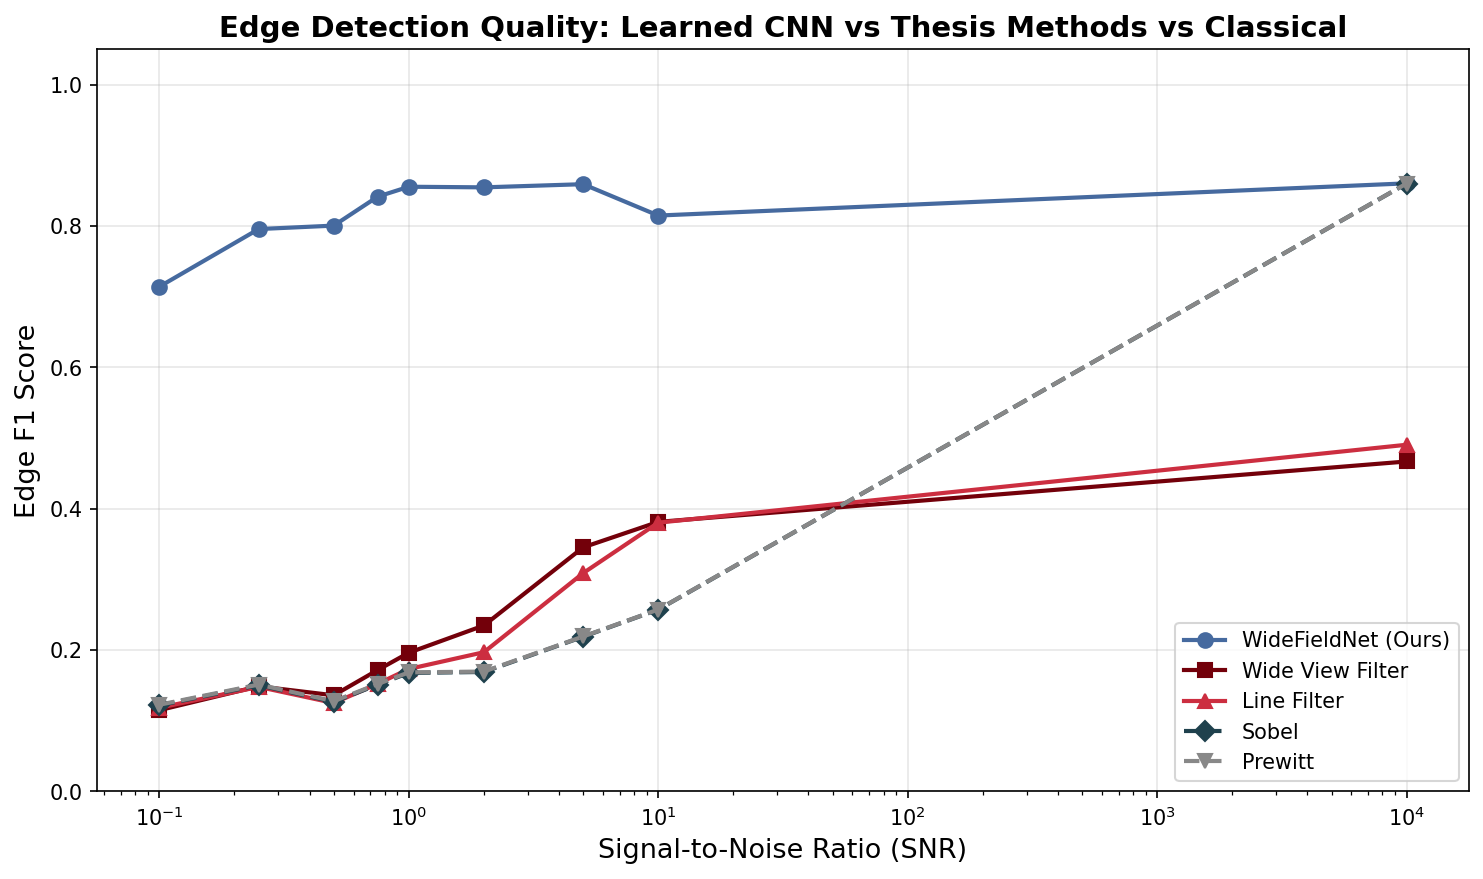
\includegraphics[width=\textwidth]{wfn_f1_comparison.png}
    \end{column}
    \begin{column}{0.43\textwidth}
      \vspace{0.5em}
      WideFieldNet dominated across all SNR levels on synthetic data.

      \vspace{0.4em}
      But the WVF/LF scores were \textbf{far below} what Bagan reported. This prompted a deeper investigation into the filter parameters.
    \end{column}
  \end{columns}
\end{frame}

\begin{frame}{CNN vs WVF/LF on Synthetic Data}
  \begin{center}
    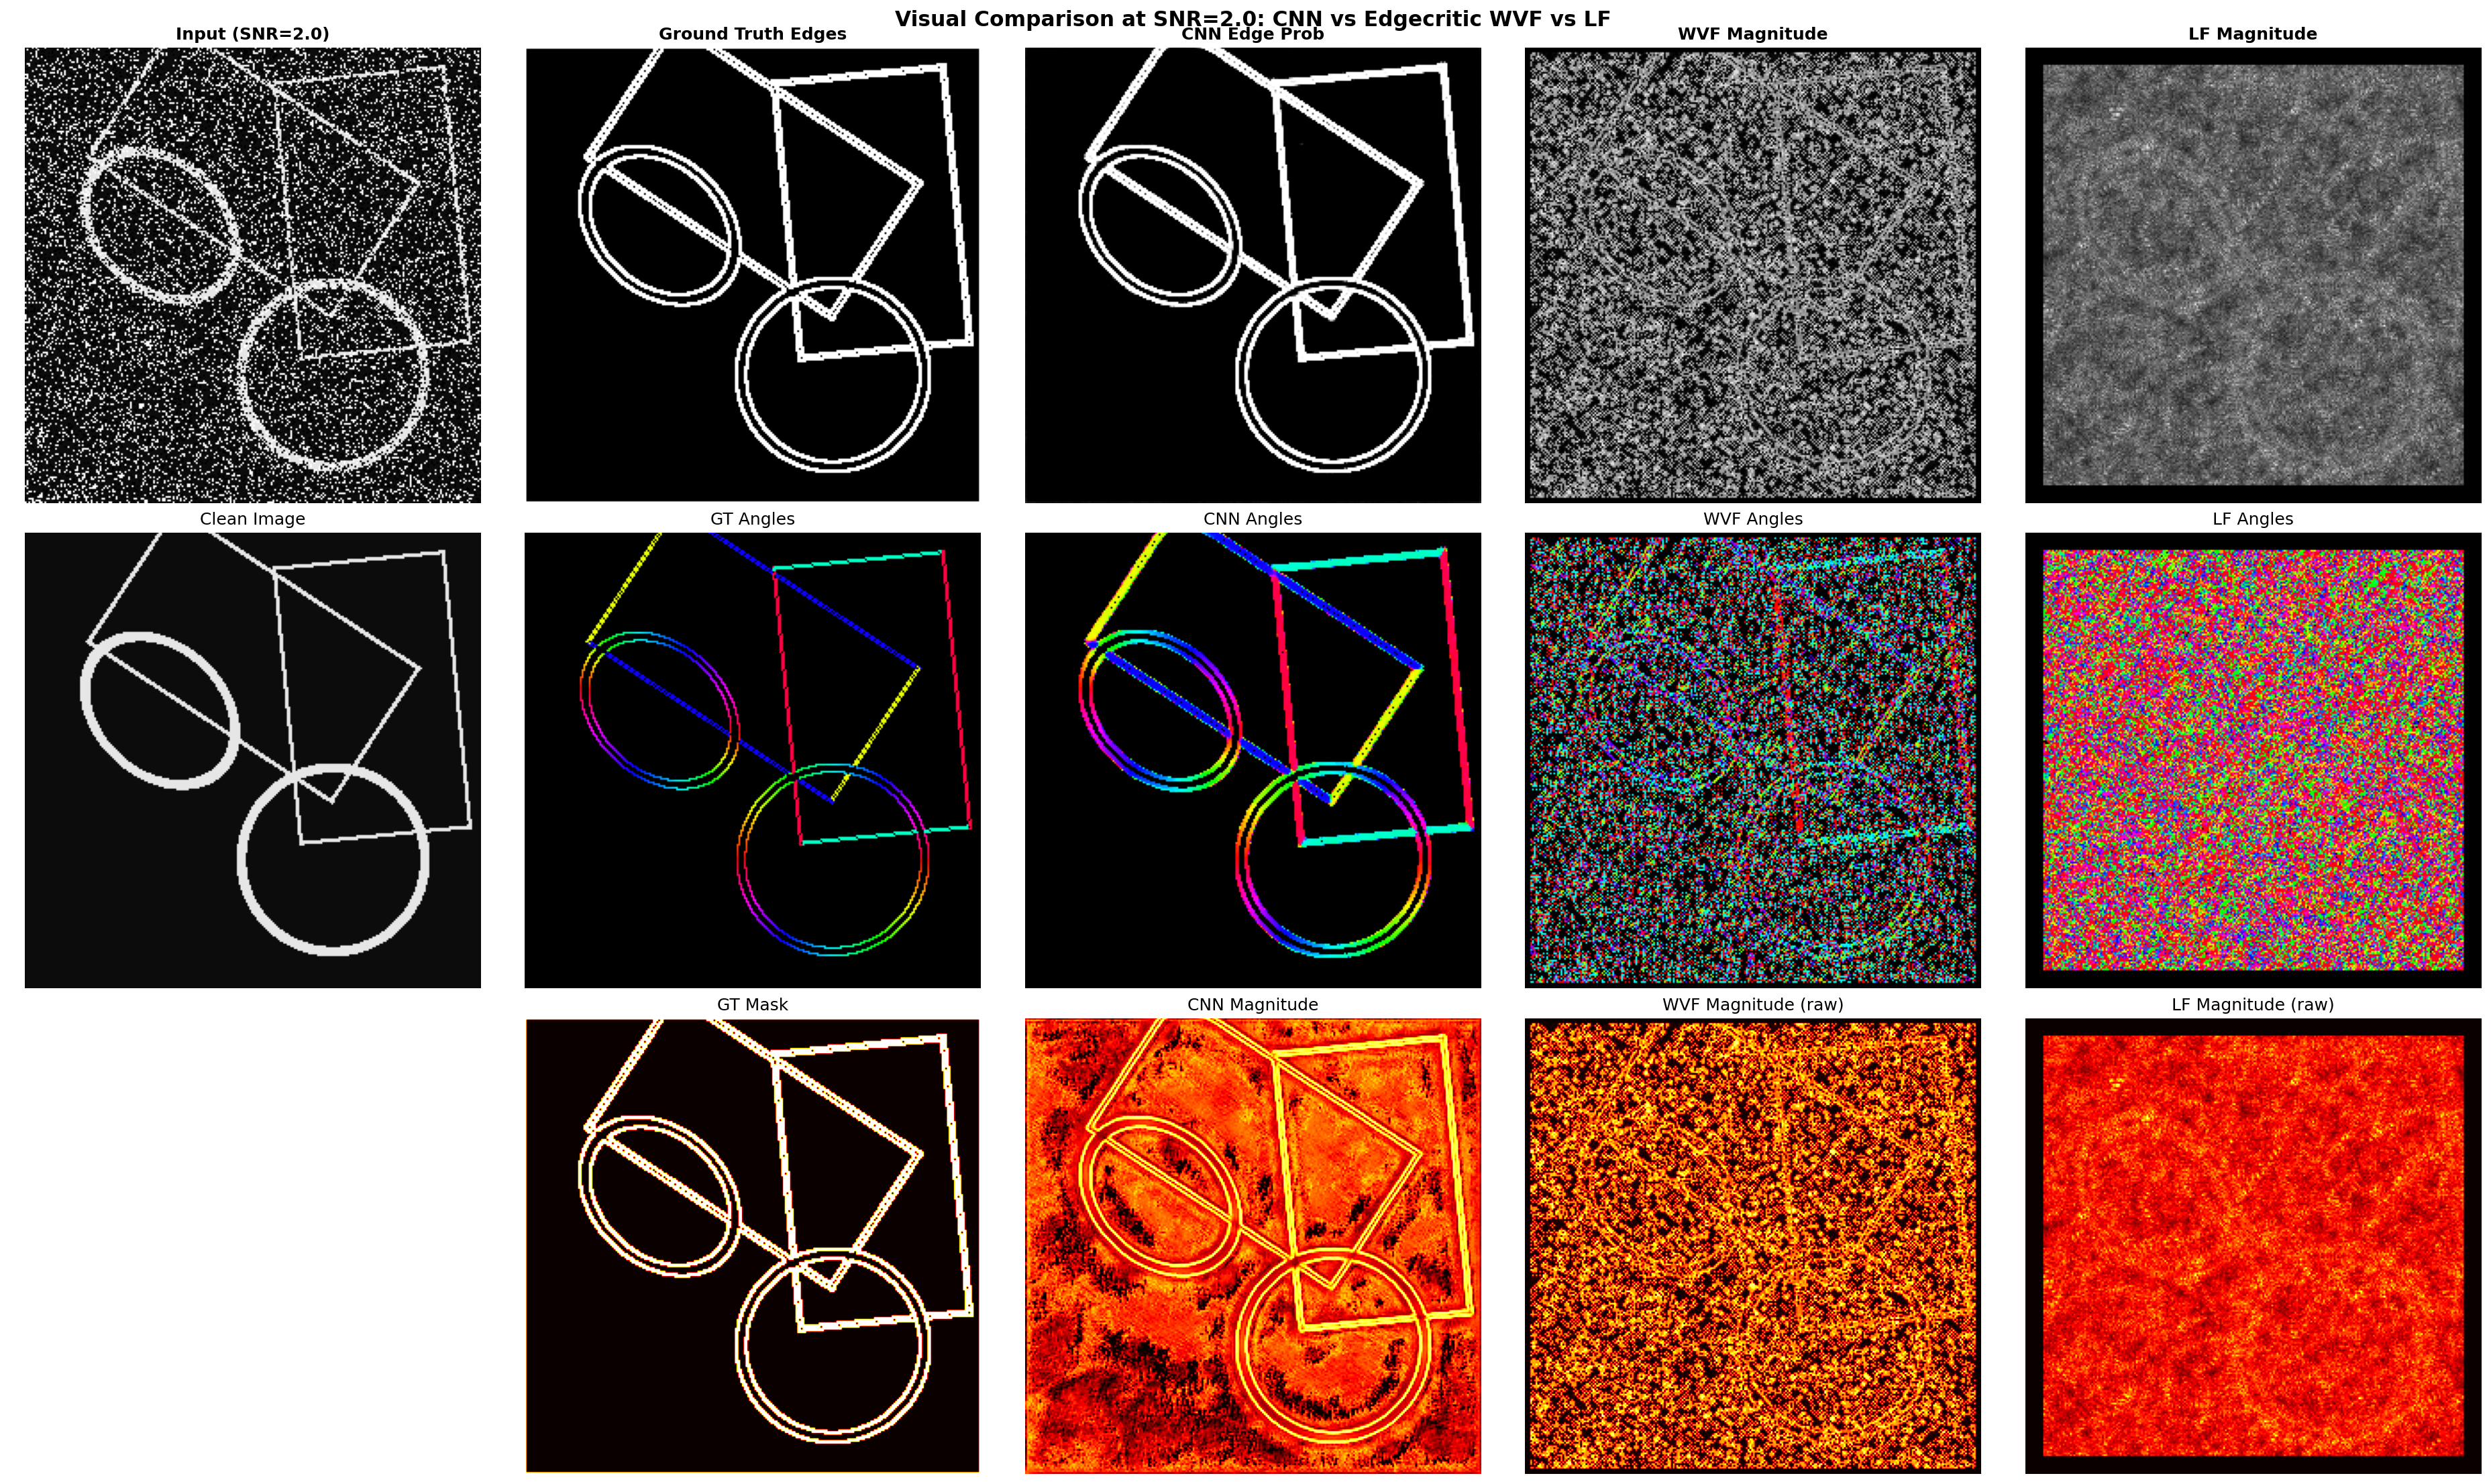
\includegraphics[width=0.85\textwidth, height=0.7\textheight, keepaspectratio]{wfn_vs_wvf_lf_visual.png}
  \end{center}

  \vspace{0.1em}
  {\scriptsize At SNR=2.0, WideFieldNet (col 3) recovers clean edges and angles. WVF/LF magnitude maps (cols 4--5) are dominated by noise. This gap was too large to accept without scrutiny.}
\end{frame}

\begin{frame}{Four Reports of Investigation}
  The CNN results led to a systematic critique of the WVF/LF filters.

  \vspace{0.3em}
  \begin{enumerate}
    \item \textbf{Parameter ablation} --- Bagan's published parameters ($N_p{=}250$, $N_s{=}18$, $d{=}4$) are suboptimal. Optimal: $N_p{=}25$, $N_s{=}4$, $d{=}2$. ODS gains of +0.01 to +0.16.
    \item \textbf{Benchmarking} --- Optimized WVF beats all 54 classical operators. DL models are 0.09 ODS higher but 400$\times$ slower.
    \item \textbf{Noise robustness} --- Bagan's large $N_p$ was optimal for \textit{noisy underwater data}. Optimal $N_p$ scales inversely with SNR (25$\to$400).
    \item \textbf{Statistical validation} --- Nonparametric tests confirm all claims. BSDS500 is an outlier dataset ($\rho{<}0.17$ with others).
  \end{enumerate}

  \vspace{0.3em}
  This also led to developing a \textbf{GPU-accelerated ASF} reformulation --- collapsing the LF pipeline into a single fused convolution (\textbf{24$\times$} speedup, \textbf{311$\times$} VRAM reduction).
\end{frame}

\begin{frame}{ASF Speedup Results}
  \begin{center}
    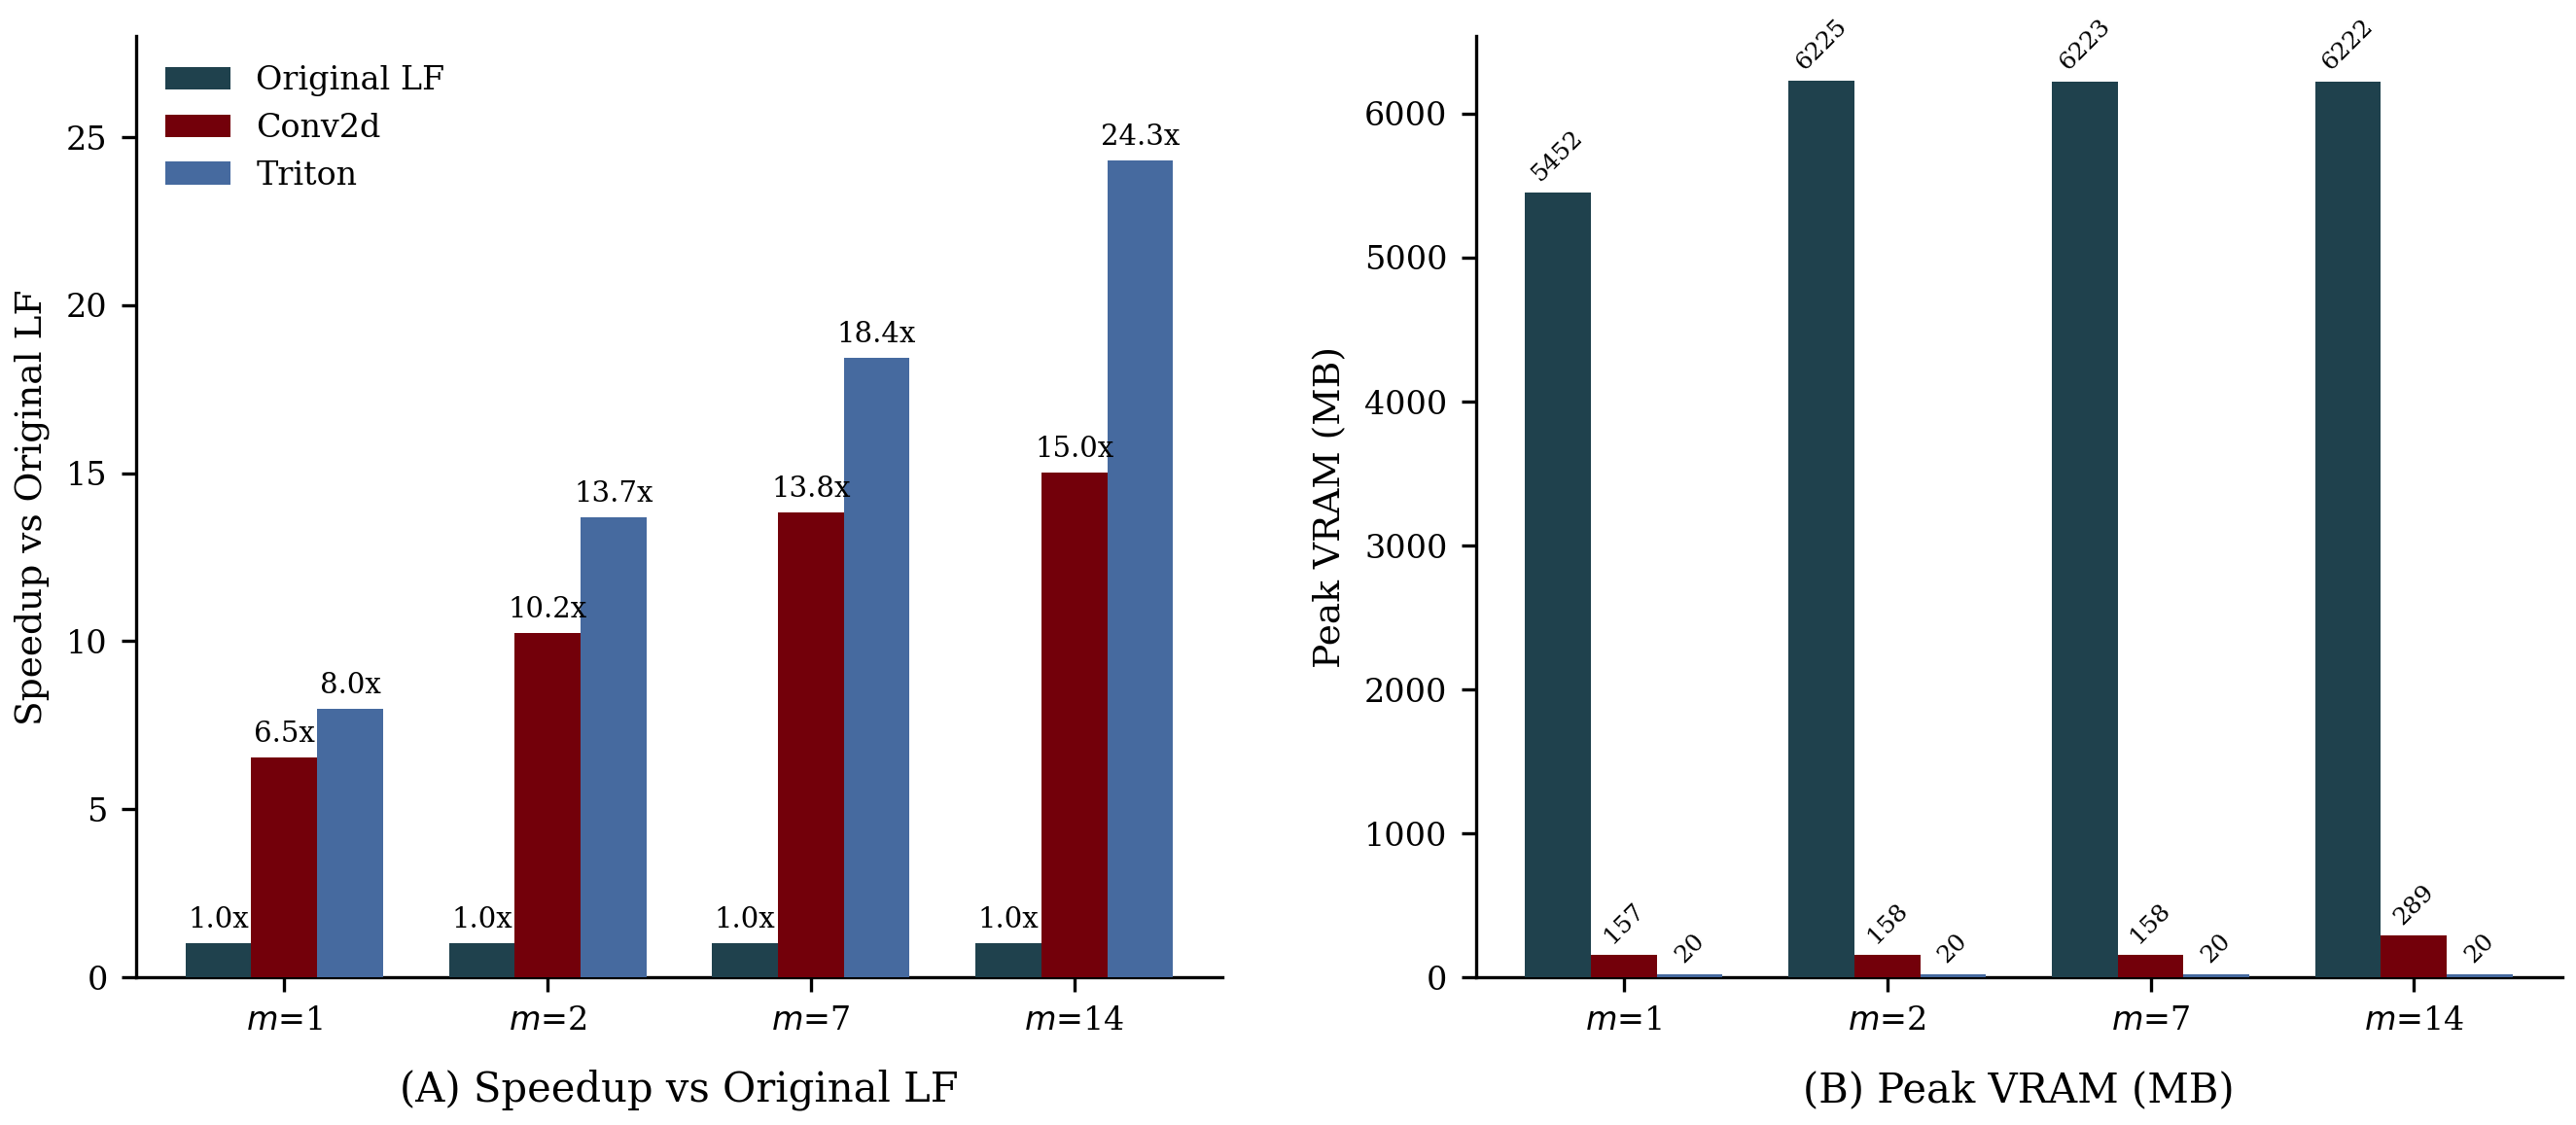
\includegraphics[width=0.88\textwidth]{asf_speedup_vram.png}
  \end{center}

  \vspace{0.2em}
  {\small \textbf{24$\times$} wall-clock speedup at $m{=}14$, \textbf{311$\times$} VRAM reduction (6.2~GB $\to$ 20~MB). The ASF reformulation fuses overlapping virtual-pixel neighborhoods into a single stencil per orientation.}
\end{frame}

\begin{frame}{But the Fused Weights Are Wasteful}
  Examining the fused stencil weights revealed a deeper issue.

  \vspace{0.5em}
  The ASF is faster than the naive LF, but the \textit{stencil it produces} is irregular. Many pixels carry \textbf{near-zero} or \textbf{cancelled} weight due to overlapping neighborhood contributions.

  \vspace{0.5em}
  \begin{alertblock}{Key question}
    The polynomial fitting, pseudoinverse, and deduplication pipeline produces a weighted kernel. Can we define the kernel shape \textit{directly} and assign weights geometrically, skipping the polynomial machinery entirely?
  \end{alertblock}
\end{frame}

\begin{frame}{The Overlap Problem}
  When virtual pixel neighborhoods overlap and their contributions are fused, many pixels receive \textbf{near-zero} or \textbf{cancelled} weights.

  \vspace{0.3em}
  \begin{alertblock}{Observation}
    At $m{=}7$, $N_p{=}20$: the stencil uses \textbf{91 pixels}, but most carry negligible weight. The polynomial fit and deduplication produce \textit{irregular, unpredictable} weight distributions.
  \end{alertblock}

  \vspace{0.3em}
  Can we define the kernel shape \textit{directly} and assign weights geometrically?
\end{frame}

\begin{frame}{Kernel Weight Comparison}
  \begin{center}
    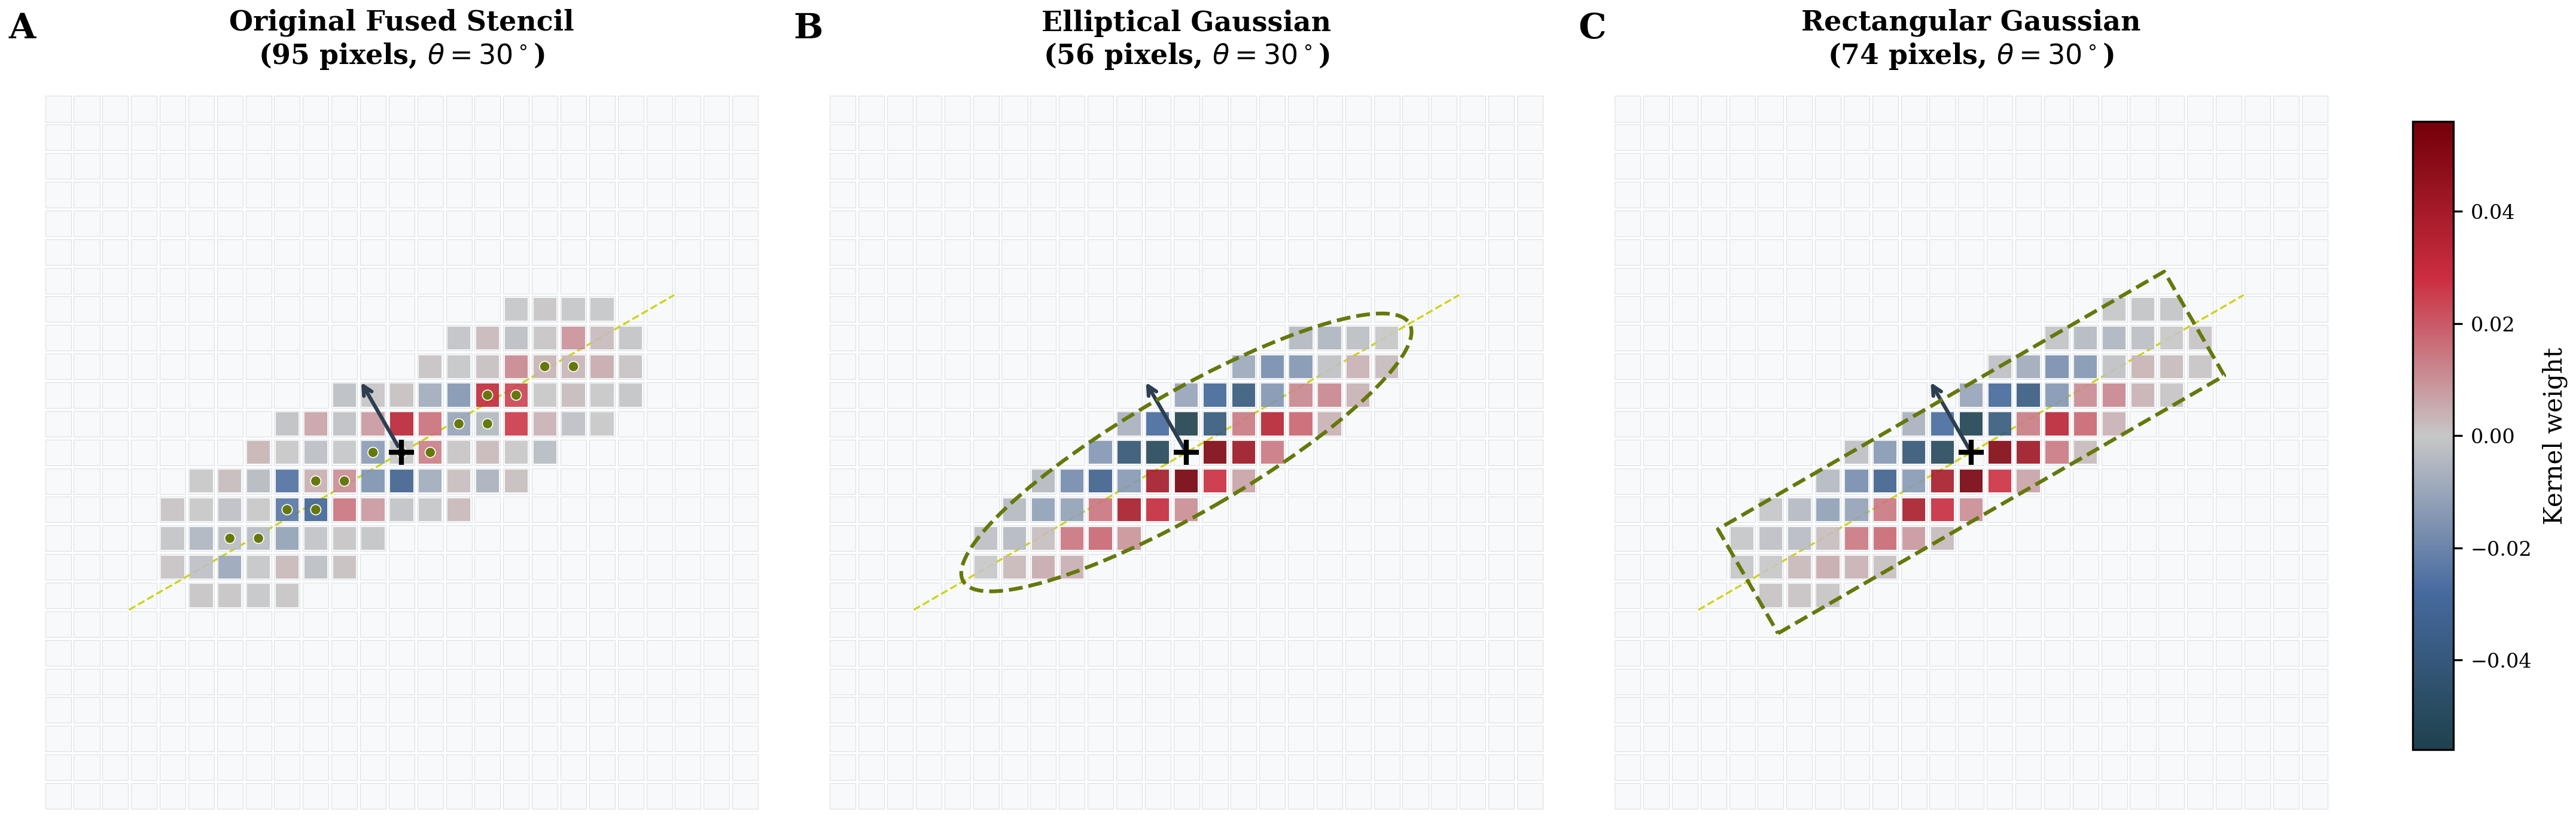
\includegraphics[width=0.95\textwidth]{fig1b_kernel_comparison.png}
  \end{center}

  \vspace{0.3em}
  {\small \textbf{A:} Fused stencil (95 px, irregular, scattered outliers).
  \textbf{B:} Elliptical Gaussian (56 px, smooth).
  \textbf{C:} Rectangular Gaussian (74 px, clean boundary). All matched to the same effective aspect ratio.}
\end{frame}

% ============================================================
\sectionsubtitle{Elliptical and rectangular Gaussian kernels}
\section{Geometric Kernel Designs}

\begin{frame}{Two Geometric Alternatives}
  Both designs share the same core structure. Rotate pixel coordinates into the kernel frame, apply a distribution, and multiply by the derivative profile.

  \vspace{0.3em}
  \begin{columns}[T]
    \begin{column}{0.48\textwidth}
      \begin{block}{Elliptical Gaussian}
        Boundary: $\displaystyle\frac{u^2}{\sigma_a^2} + \frac{v^2}{\sigma_c^2} \leq 9$

        \vspace{0.3em}
        Weight: $K = -v \cdot \exp\!\Bigl(-\frac{u^2}{2\sigma_a^2} - \frac{v^2}{2\sigma_c^2}\Bigr)$

        \vspace{0.3em}
        \begin{itemize}
          \item Smooth falloff at boundary
          \item Fewest active pixels
          \item Best at high noise
        \end{itemize}
      \end{block}
    \end{column}
    \begin{column}{0.48\textwidth}
      \begin{block}{Rectangular Gaussian}
        Boundary: $|u| \leq h_a$, $|v| \leq h_c$

        \vspace{0.3em}
        Weight: same Gaussian $\times$ $(-v)$, clipped to rectangle

        \vspace{0.3em}
        \begin{itemize}
          \item Hard boundary, Gaussian inside
          \item More active pixels than ellipse
          \item Slight edge on clean images
        \end{itemize}
      \end{block}
    \end{column}
  \end{columns}

  \vspace{0.3em}
  {\small Every pixel gets \textbf{exactly one weight}, determined solely by its geometric position. No polynomial fitting, no pseudoinverse, no overlapping neighborhoods, no cancellation.}
\end{frame}

\begin{frame}{Stencil Weights by Orientation}
  \begin{center}
    
\includegraphics[width=0.92\textwidth]{fig3_stencil_orientations.png}
  \end{center}

  \vspace{0.2em}
  {\small Top: original fused stencil (91--97 px, irregular shape). Middle: elliptical Gaussian (smooth, compact). Bottom: rectangular Gaussian (consistent rectangular boundary). All matched to the same effective aspect ratio.}
\end{frame}

% ============================================================
\sectionsubtitle{3$\times$ faster, same accuracy}
\section{Performance}

\begin{frame}{Speed Comparison}
  All three filters at matched parameters ($\sigma{=}2.0$, 36 orientations, 640$\times$427 image). Median of 10 runs.

  \vspace{0.5em}
  \begin{table}
    \centering
    \begin{tabular}{lccc}
      \toprule
      \textbf{Filter} & \textbf{Time (ms)} & \textbf{Speedup} & \textbf{ODS F-score} \\
      \midrule
      Original (fused stencil) & 4,013 & 1.0$\times$ & 0.4221 \\
      Elliptical Gaussian      & 1,201 & \textbf{3.3$\times$} & 0.4211 \\
      Rectangular Gaussian     & 1,424 & \textbf{2.8$\times$} & 0.4220 \\
      \bottomrule
    \end{tabular}
  \end{table}

  \vspace{0.5em}
  \begin{itemize}
    \item ODS scores within 0.3\% across all three designs
    \item Elliptical is fastest due to fewest active pixels (compact elliptical mask)
    \item No polynomial fitting, no pseudoinverse, no deduplication step
  \end{itemize}
\end{frame}

\begin{frame}{Side-by-Side Filter Output}
  \begin{center}
    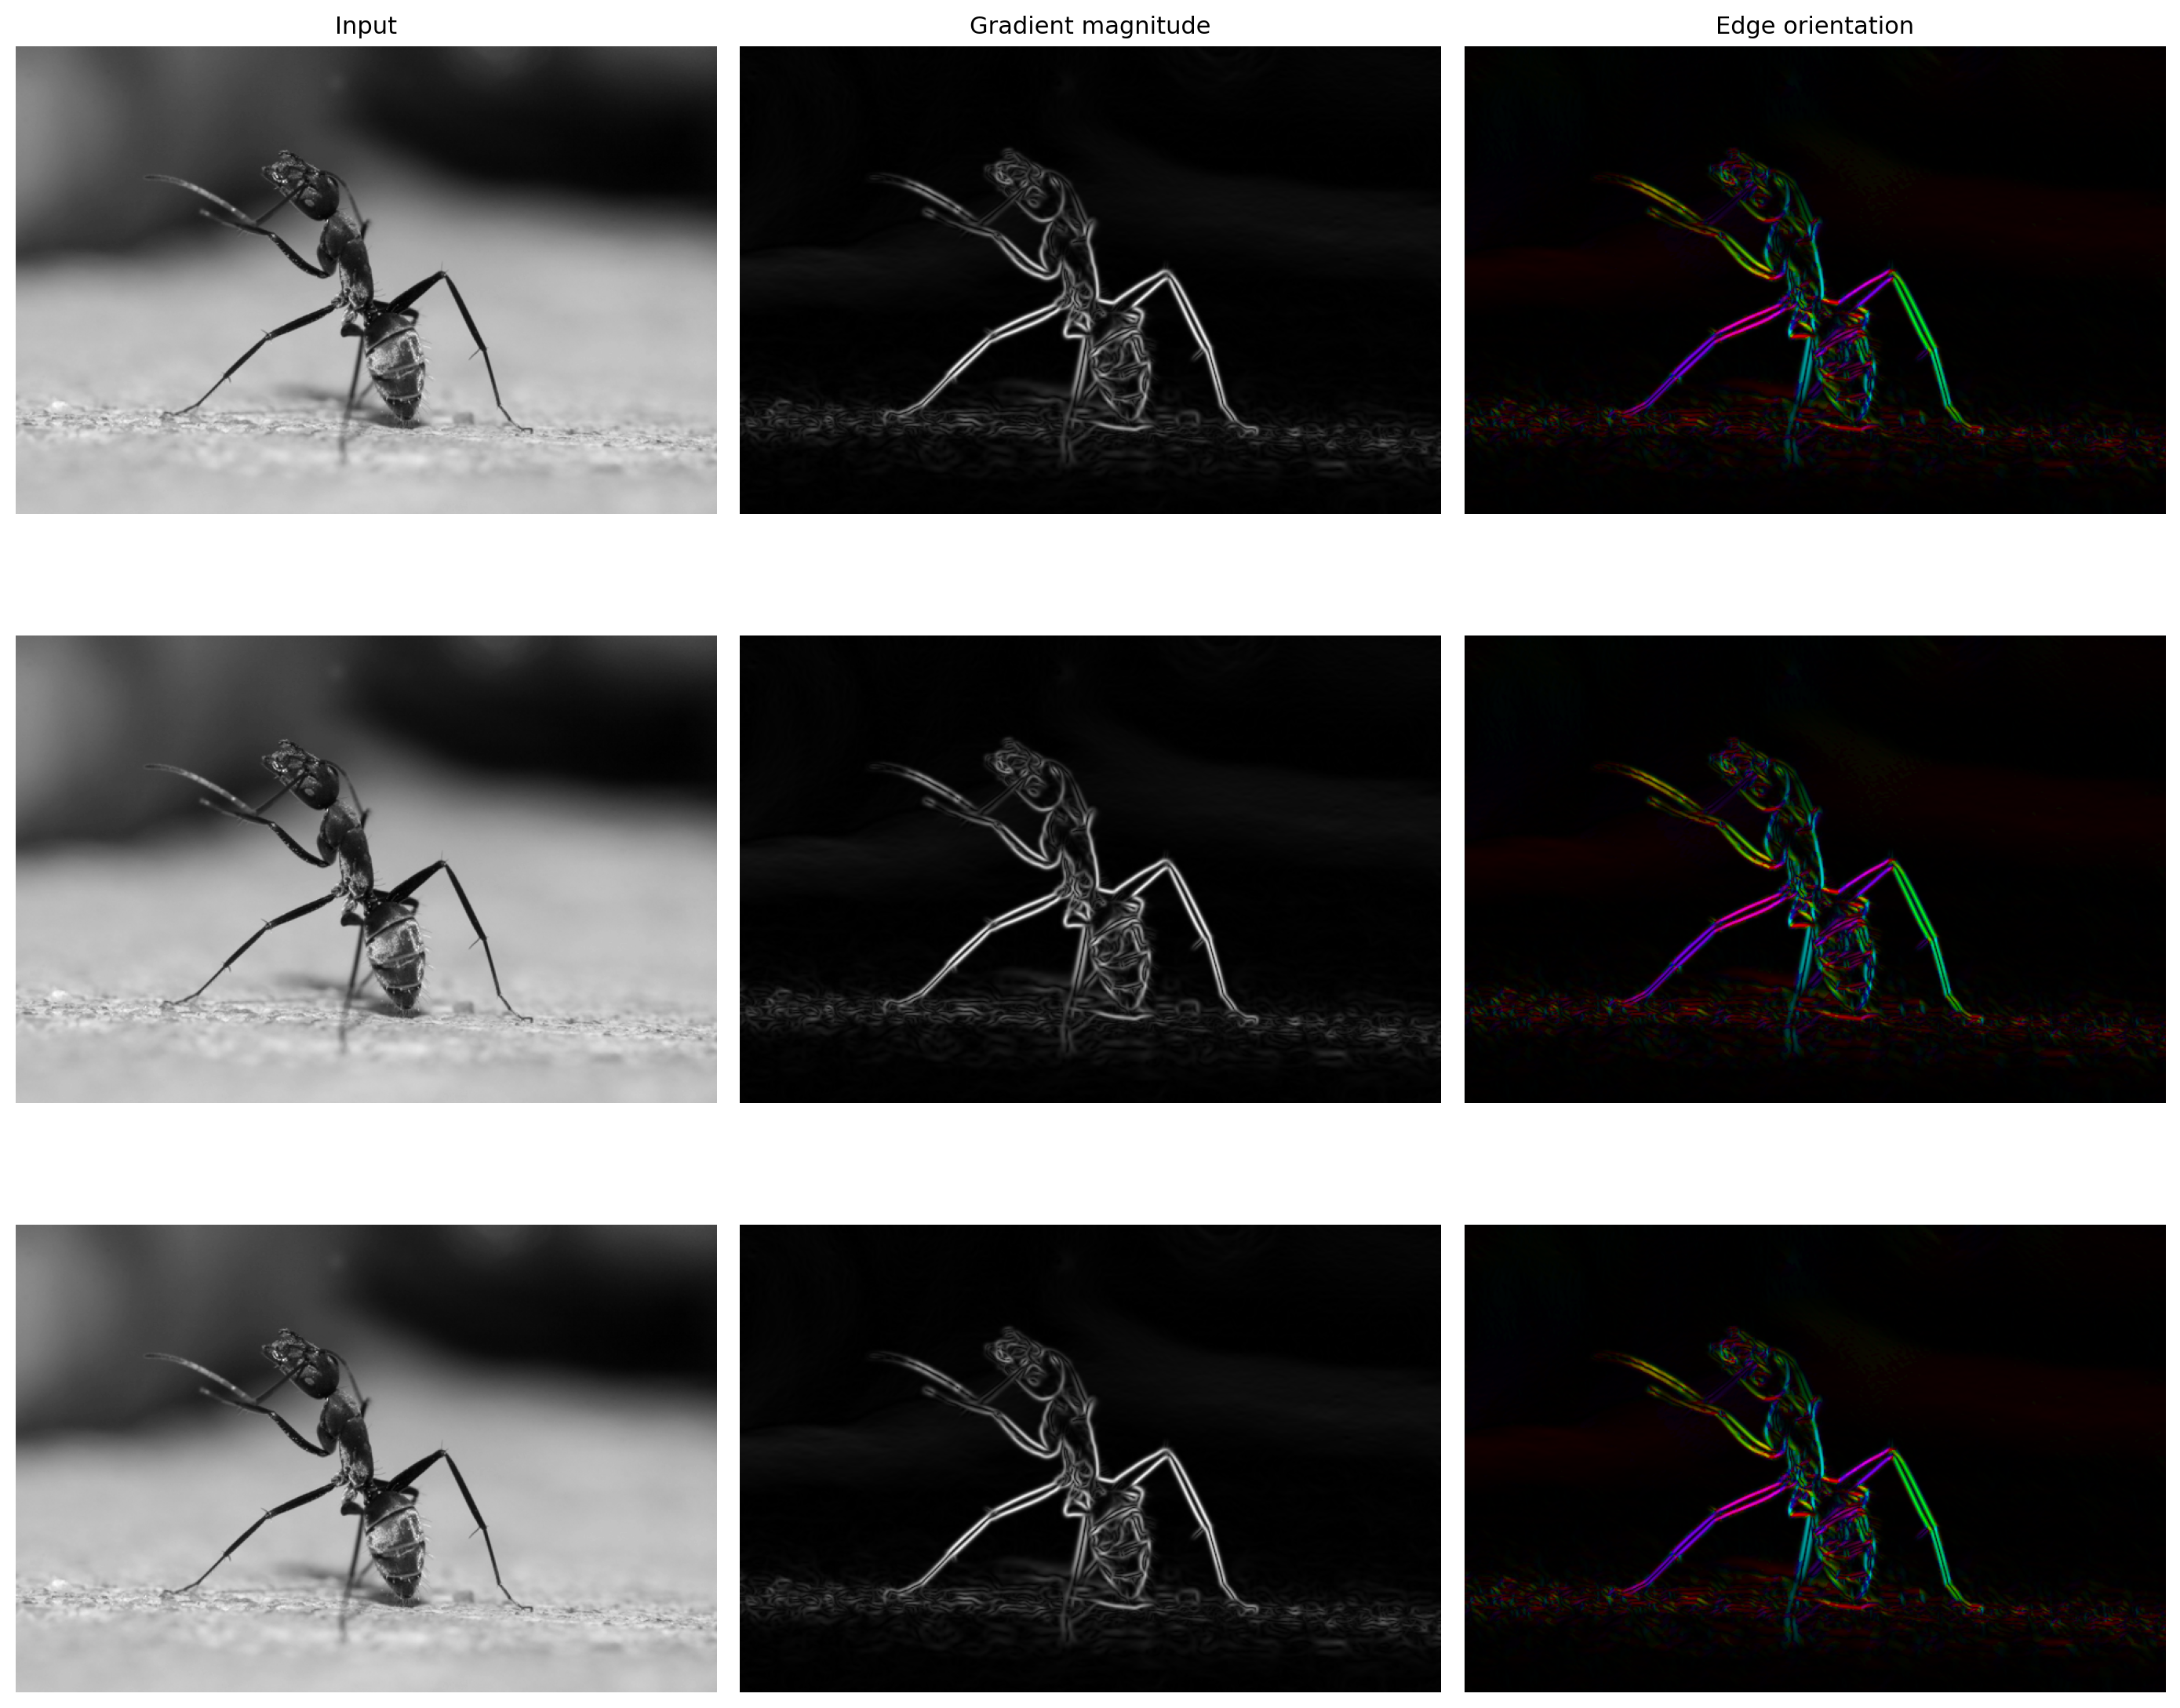
\includegraphics[width=0.82\textwidth, height=0.68\textheight, keepaspectratio]{filter_comparison.png}
  \end{center}

\end{frame}

% ============================================================
\sectionsubtitle{BSDS500 test set, 10 images}
\section{Edge Detection Results}

\begin{frame}{Clean Image Comparison}
  \begin{center}
    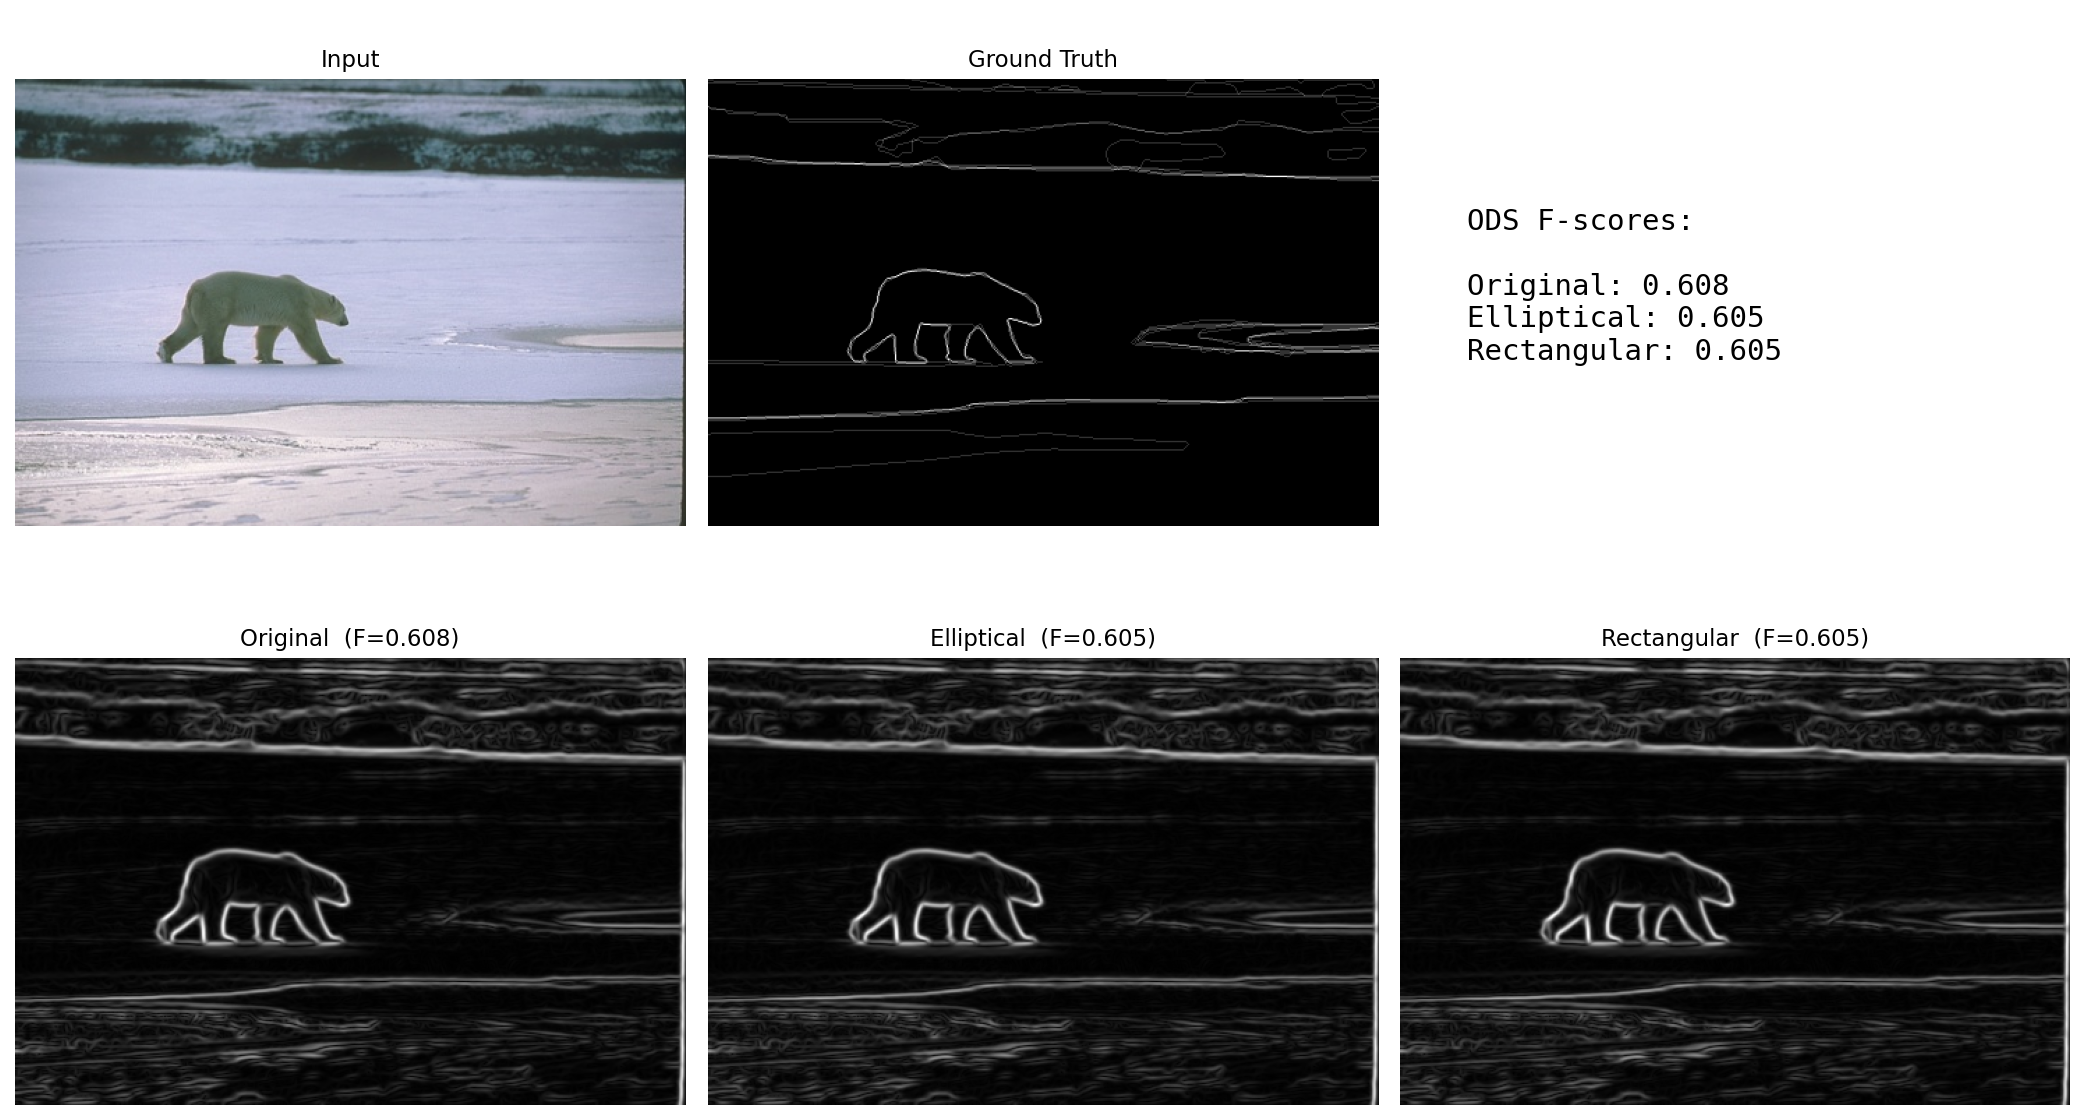
\includegraphics[width=0.85\textwidth]{BSDS500/100007.png}
  \end{center}

  \vspace{0.1em}
  {\small BSDS500 polar bear. All three filters produce nearly identical edge maps and F-scores (0.605--0.608). The geometric kernels match the polynomial-based stencil without its complexity.}
\end{frame}

\begin{frame}{Clean Image Comparison (cont.)}
  \begin{center}
    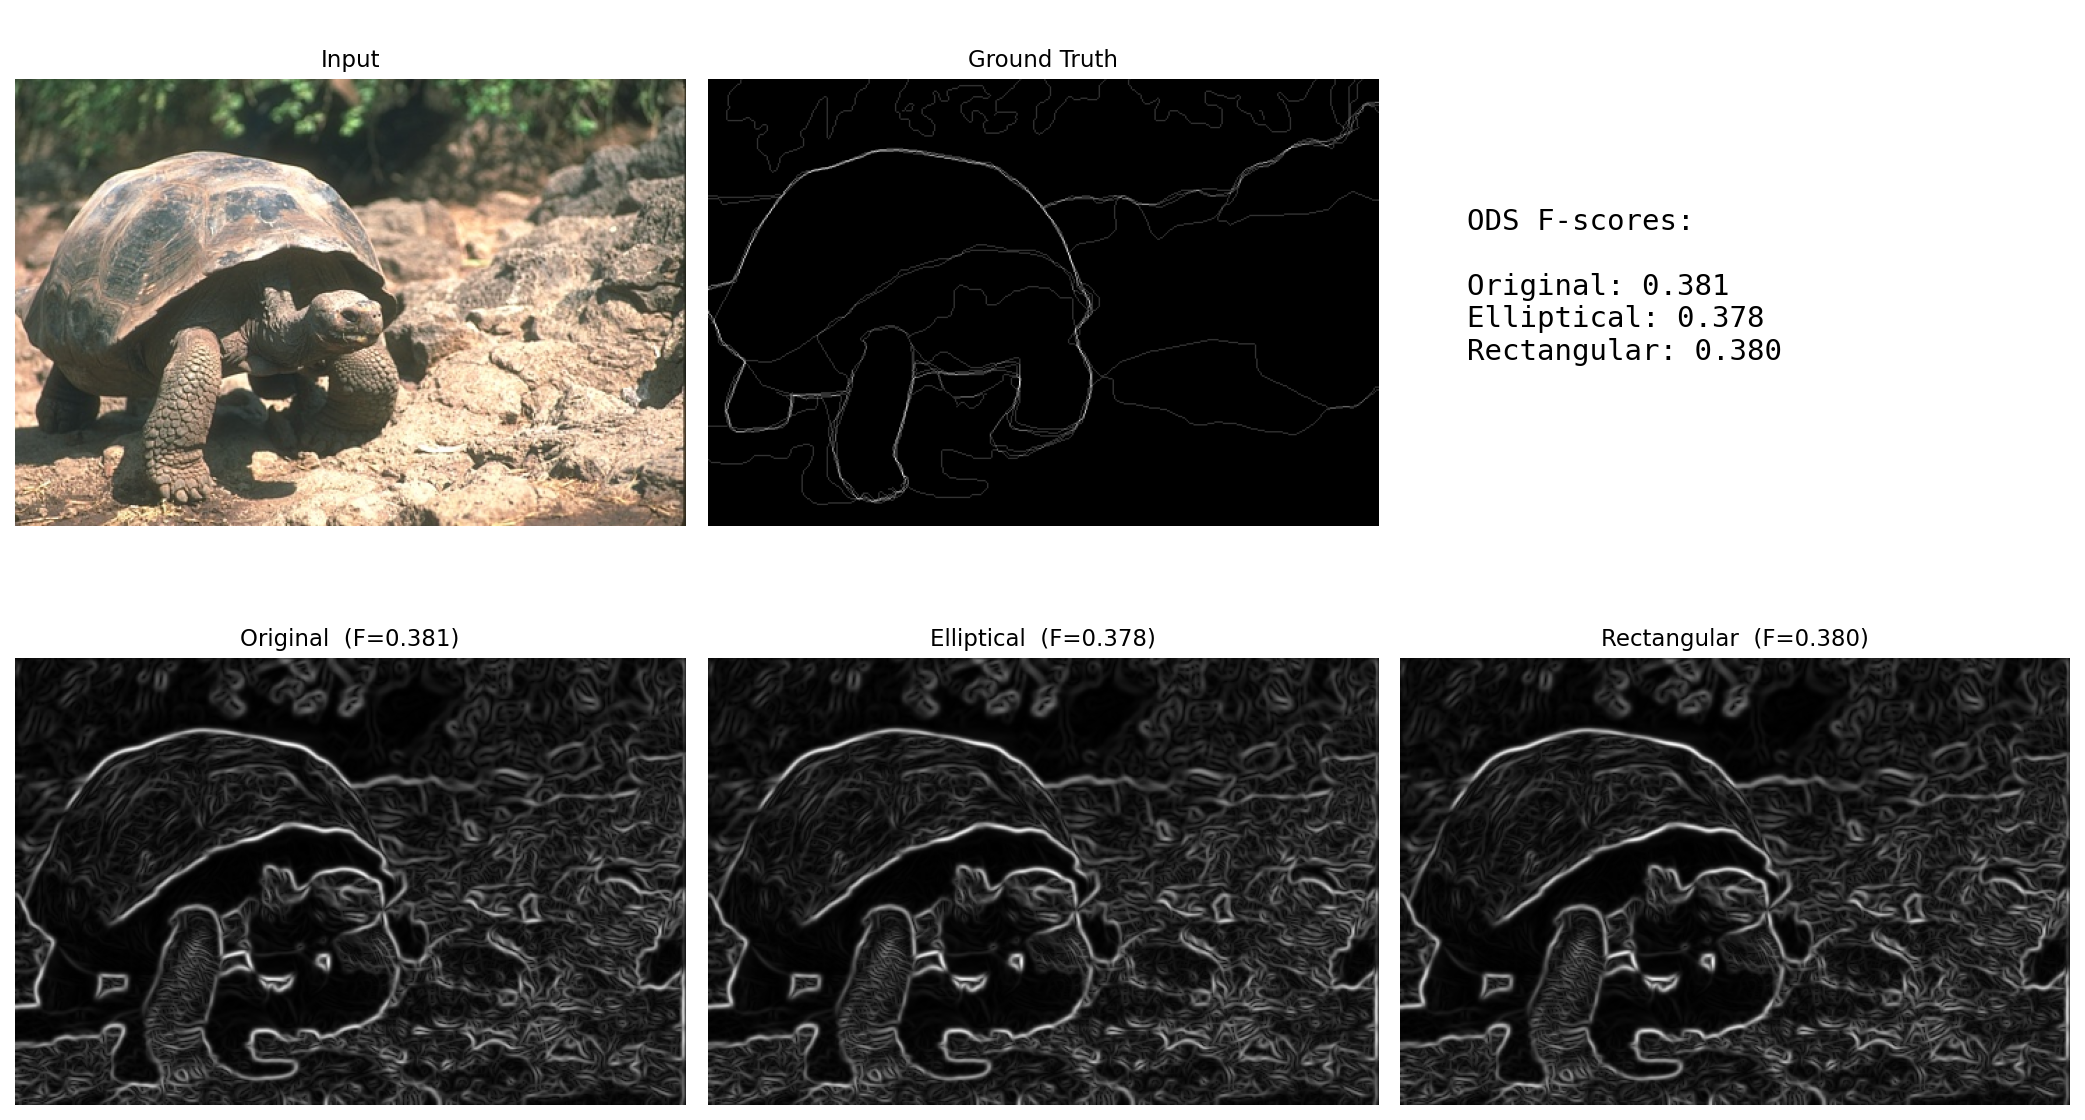
\includegraphics[width=0.85\textwidth]{BSDS500/103006.png}
  \end{center}

  \vspace{0.1em}
  {\small BSDS500 tortoise. Scores within 0.3\% (0.378--0.381). Fine-grained texture is preserved equally by all three approaches.}
\end{frame}

% ============================================================
\sectionsubtitle{Does the polynomial fit help in noise?}
\section{Noise Robustness}

\begin{frame}{SNR vs ODS}
  \begin{columns}[T]
    \begin{column}{0.65\textwidth}
      \vspace{-0.5em}
      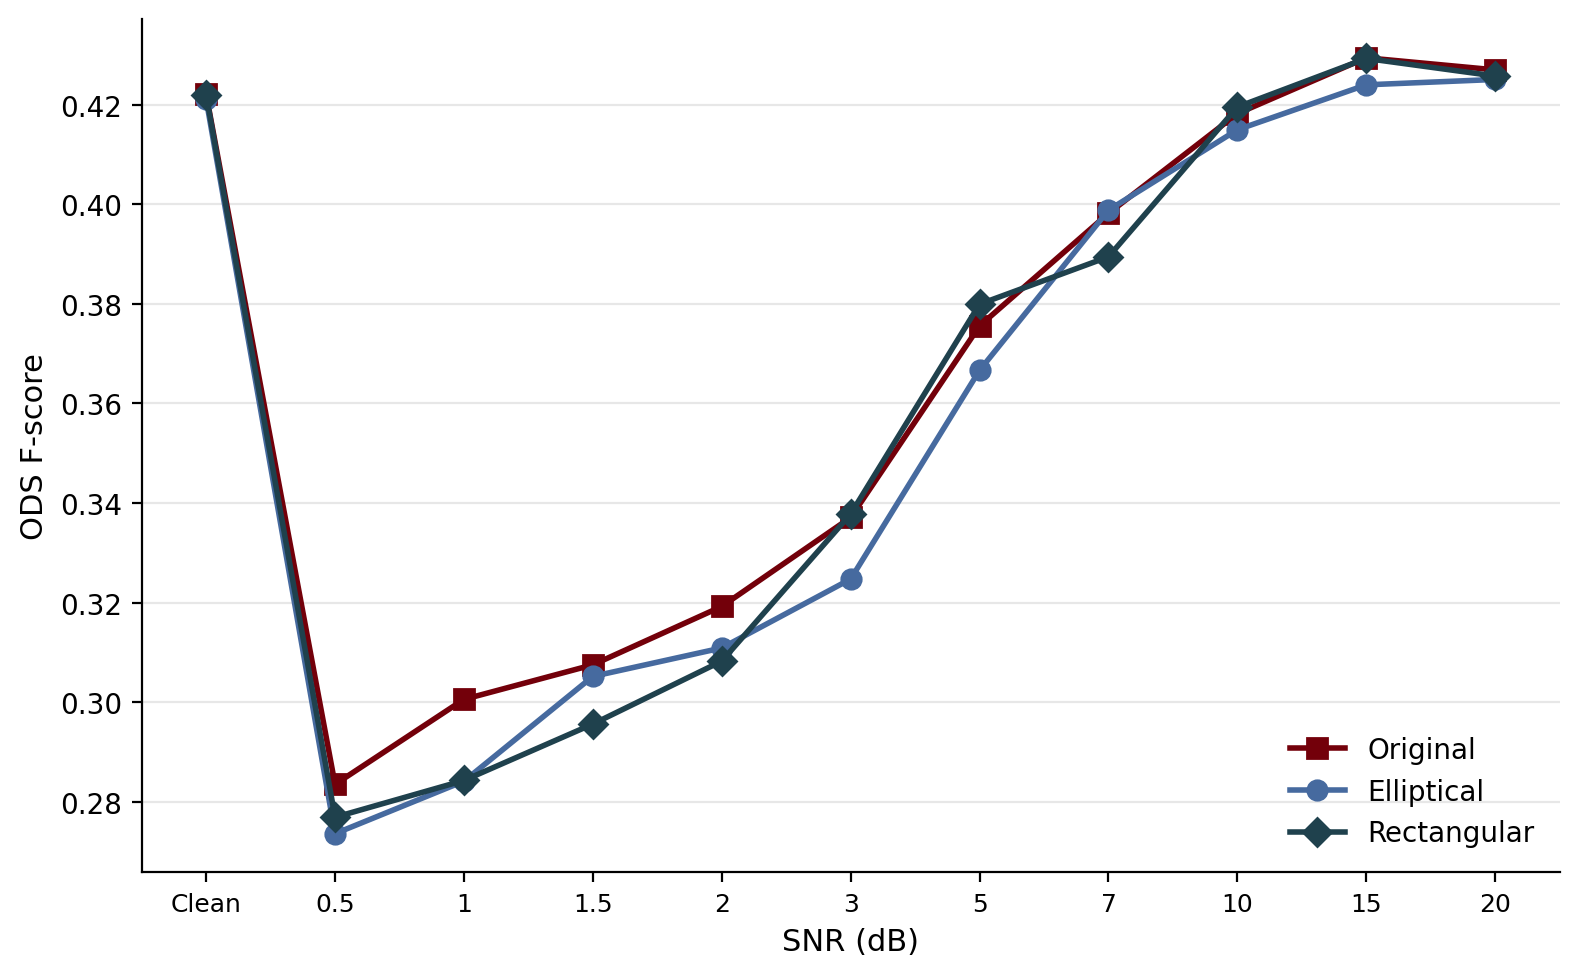
\includegraphics[width=\textwidth]{BSDS500/snr_vs_ods.png}
    \end{column}
    \begin{column}{0.33\textwidth}
      \vspace{0.5em}
      Original holds a \textbf{1--2\% ODS edge} at extreme noise (SNR $<$ 3~dB).

      \vspace{0.4em}
      Above SNR~10~dB, all three converge.

      \vspace{0.4em}
      {\color{UofSCGarnet}\textbf{Is this polynomial fitting, or just kernel size?}}
    \end{column}
  \end{columns}
\end{frame}

\begin{frame}{Scaling Up Closes the Gap}
  \begin{columns}[T]
    \begin{column}{0.65\textwidth}
      \vspace{-0.5em}
      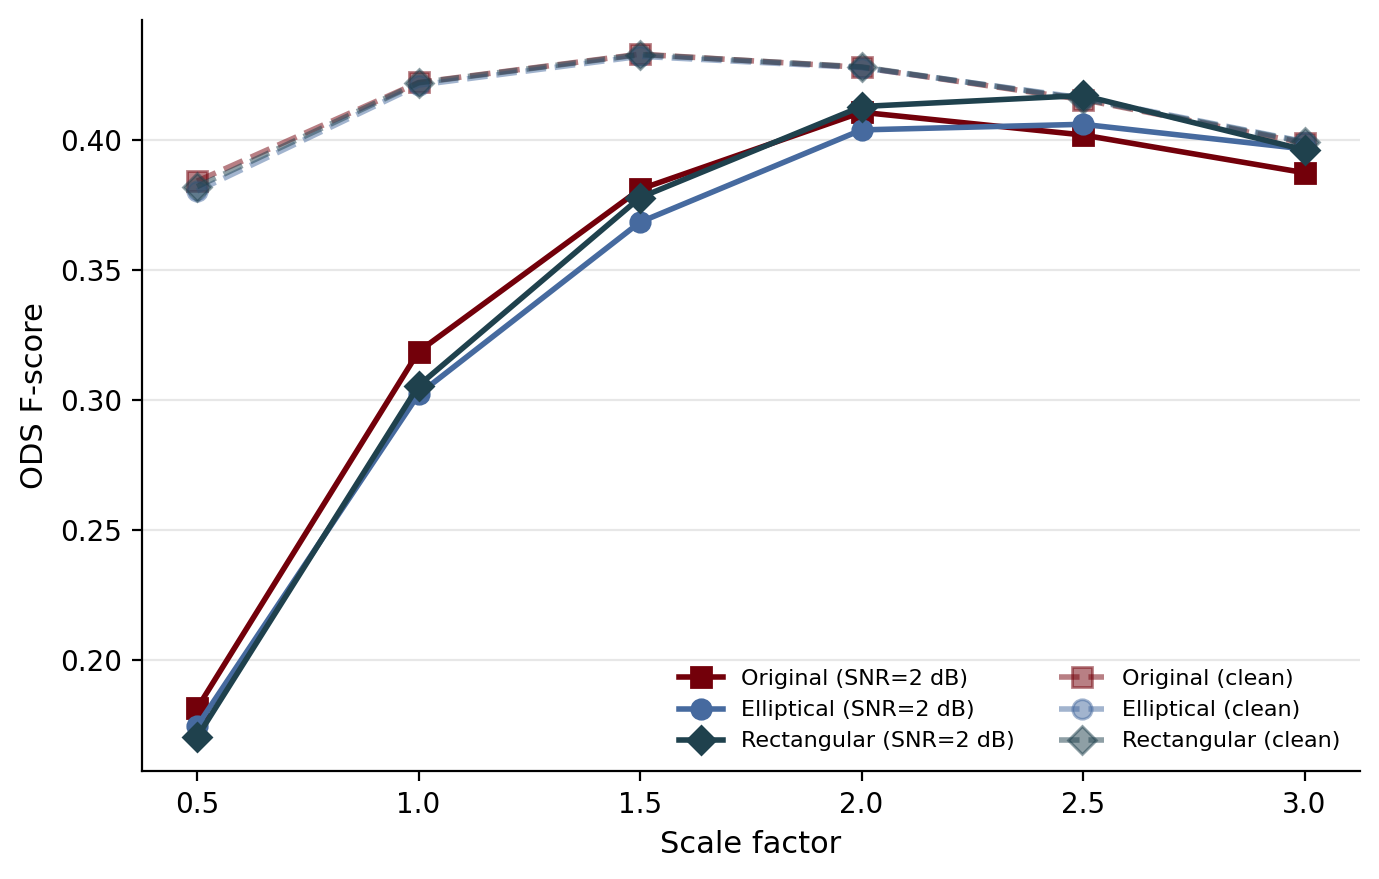
\includegraphics[width=\textwidth]{BSDS500/ods_vs_scale.png}
    \end{column}
    \begin{column}{0.33\textwidth}
      \vspace{0.5em}
      \textbf{Solid:} SNR=2~dB.\\
      \textbf{Dashed:} Clean.

      \vspace{0.4em}
      The noise advantage \textbf{disappears at scale~2.0$\times$}.

      \vspace{0.4em}
      {\color{UofSCHorseshoe}\textbf{Noise robustness is a function of kernel size, not polynomial order.}}
    \end{column}
  \end{columns}
\end{frame}

\begin{frame}{Noise Ablation: Parameters Shift}
  The ASF ablation revealed that optimal parameters change dramatically with noise level.

  \vspace{0.3em}
  \begin{table}
    \centering
    \begin{tabular}{lcccl}
      \toprule
      \textbf{Condition} & \textbf{Best $N_p$} & \textbf{Best $N_s$} & \textbf{Best $m$} & \textbf{Trend} \\
      \midrule
      Clean         & 25--40  & 3--4  & ---  & Small kernel, few orientations \\
      Gaussian SNR=4 & 65    & 3     & 5    & Larger kernel \\
      Gaussian SNR=2 & 100   & 3     & 7    & Even larger \\
      Gaussian SNR=1 & 300   & 72    & 10   & Much larger, many orientations \\
      Gaussian SNR=0.5 & 400 & 72    & 14   & Maximum size \\
      Gaussian SNR=0.3 & 400 & 36    & 14--20 & Saturated \\
      \bottomrule
    \end{tabular}
  \end{table}

  \vspace{0.3em}
  At extreme noise, the LF with $m{=}14$ uses massive elongated stencils (43$\times$15 pixels). The geometric kernels replicate this with $\sigma_a{=}7.17$, $\sigma_c{=}2.50$.
\end{frame}

\begin{frame}{Edge Maps Under Heavy Noise}
  \begin{center}
    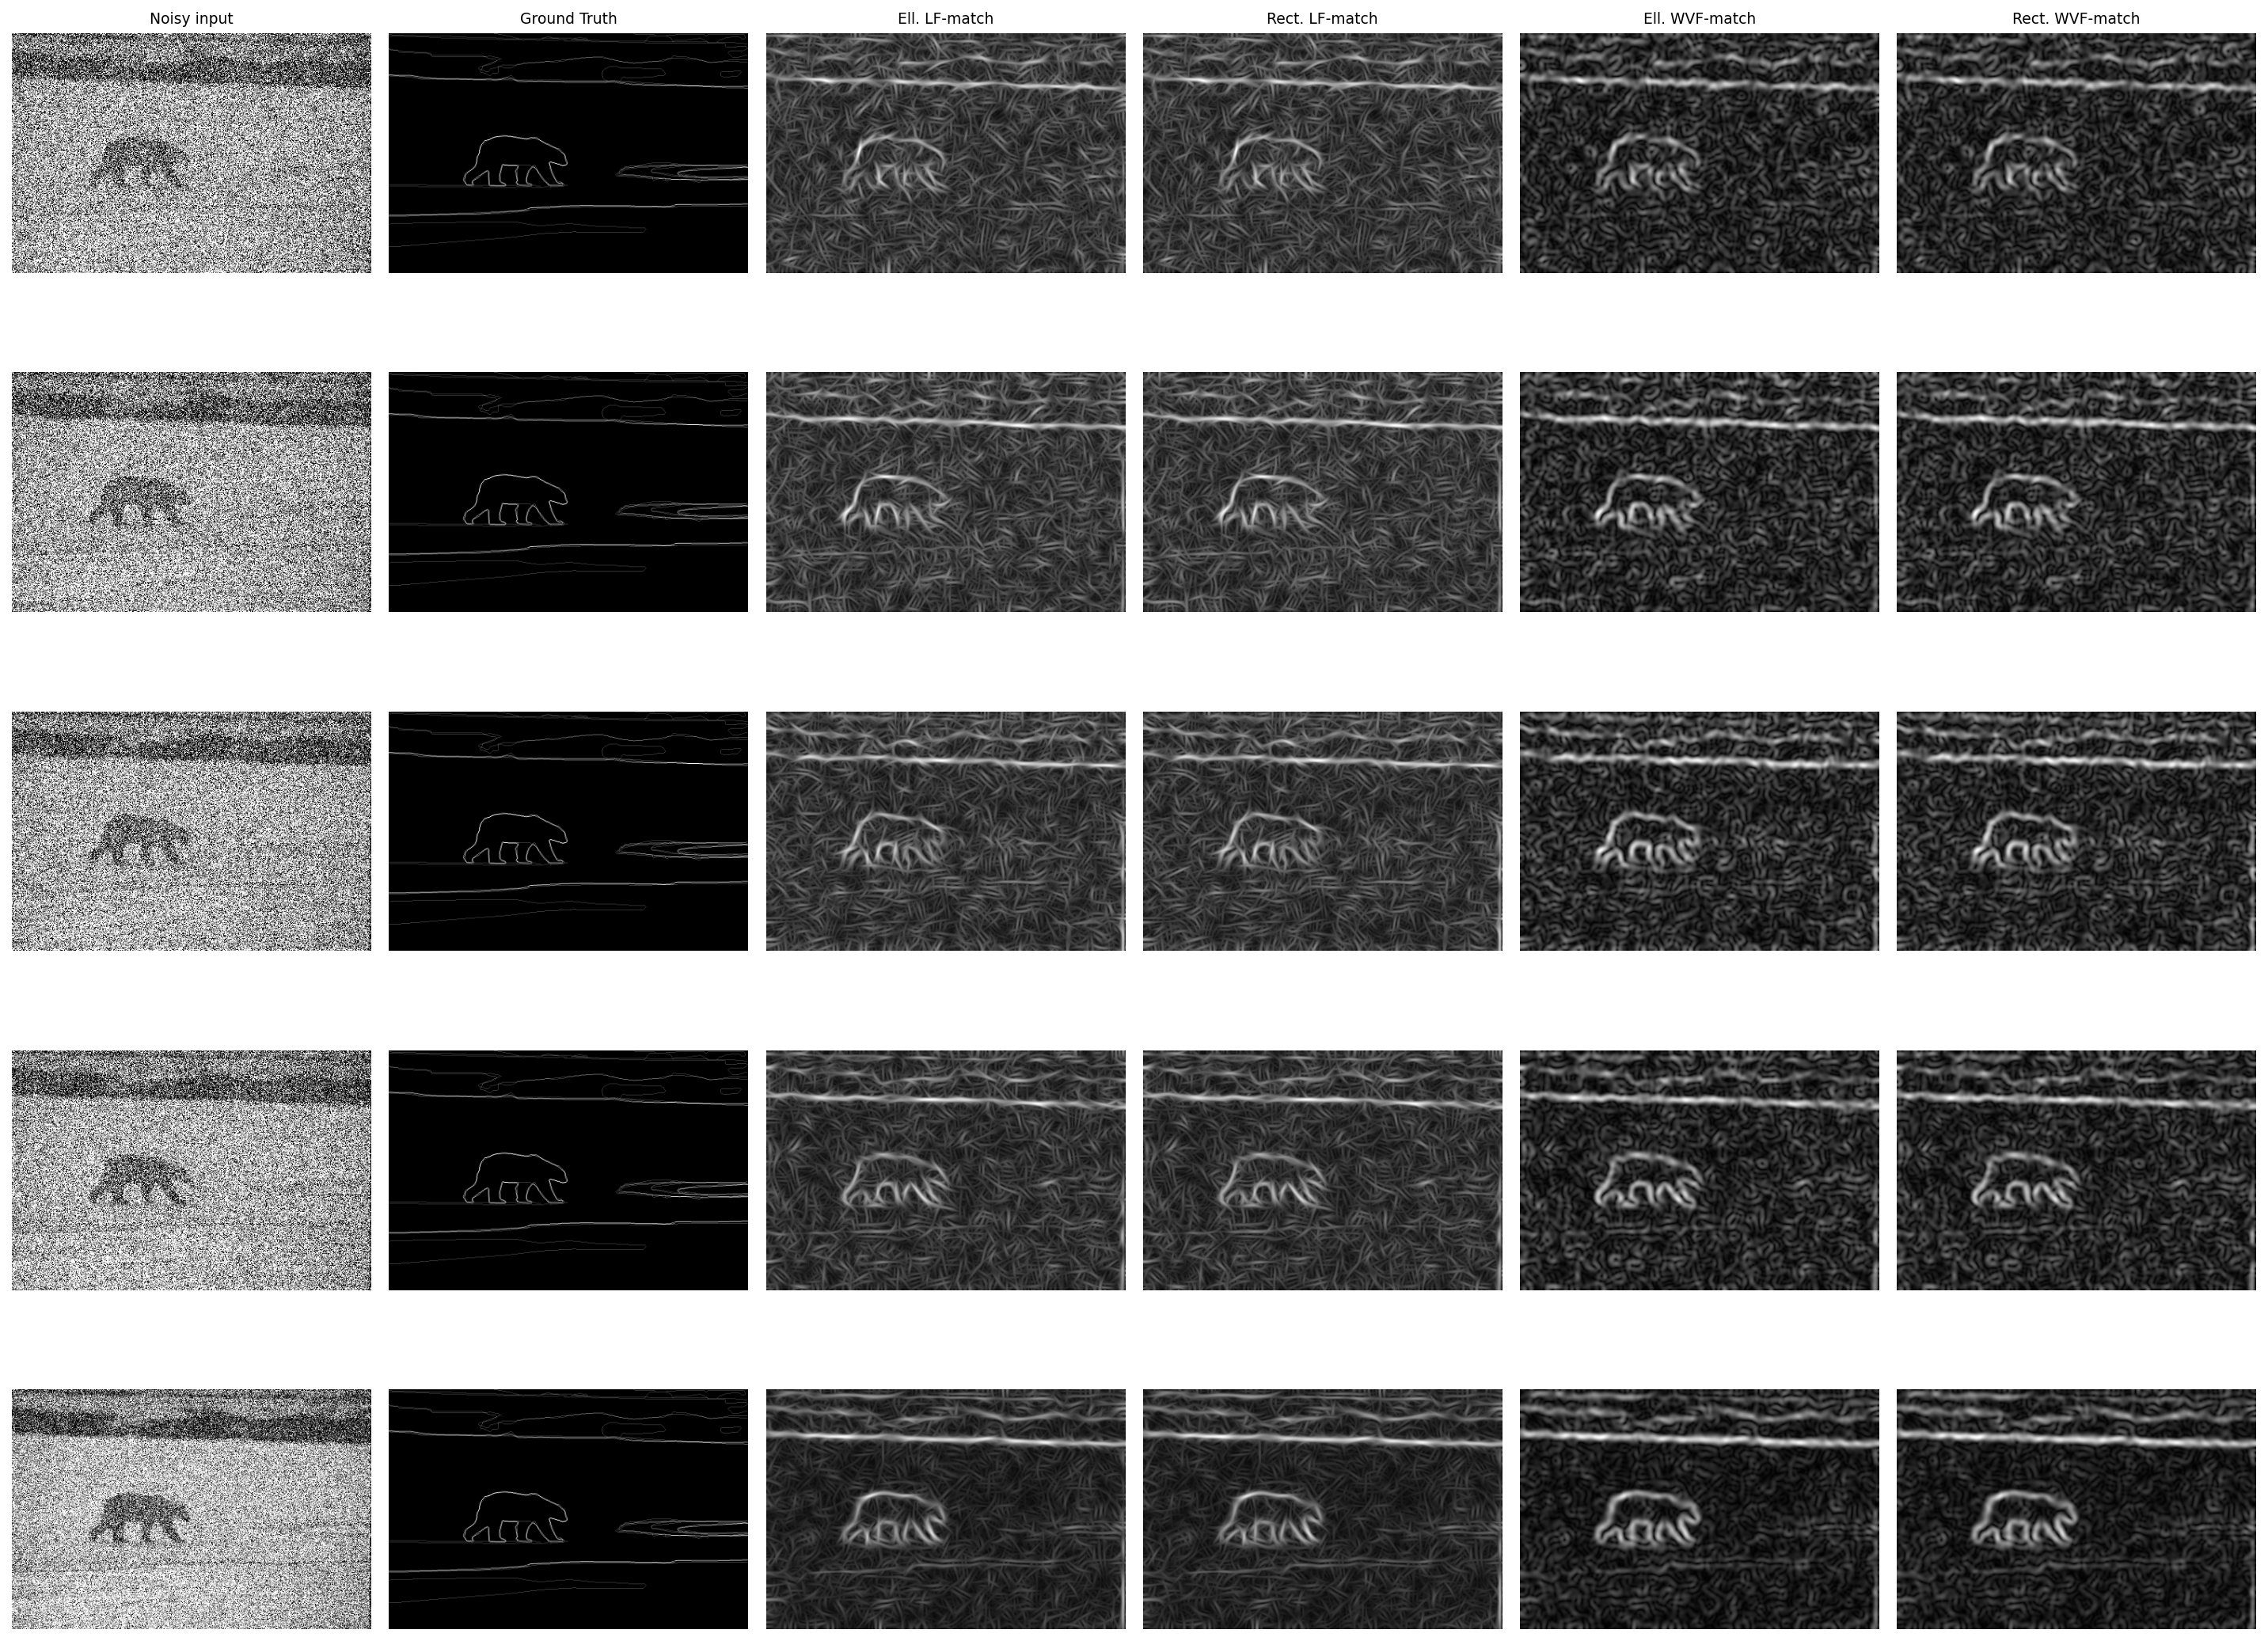
\includegraphics[width=0.92\textwidth]{BSDS500/noise_edgemaps_100007.png}
  \end{center}

  \vspace{0.1em}
  {\small Rows: SNR = 0.3, 0.5, 1.0, 2.0, 5.0~dB. LF-matched elliptical (col 3) produces the cleanest edges at extreme noise, outperforming the circular WVF-matched designs (cols 5--6).}
\end{frame}

\begin{frame}{Edge Maps Under Heavy Noise (cont.)}
  \begin{center}
    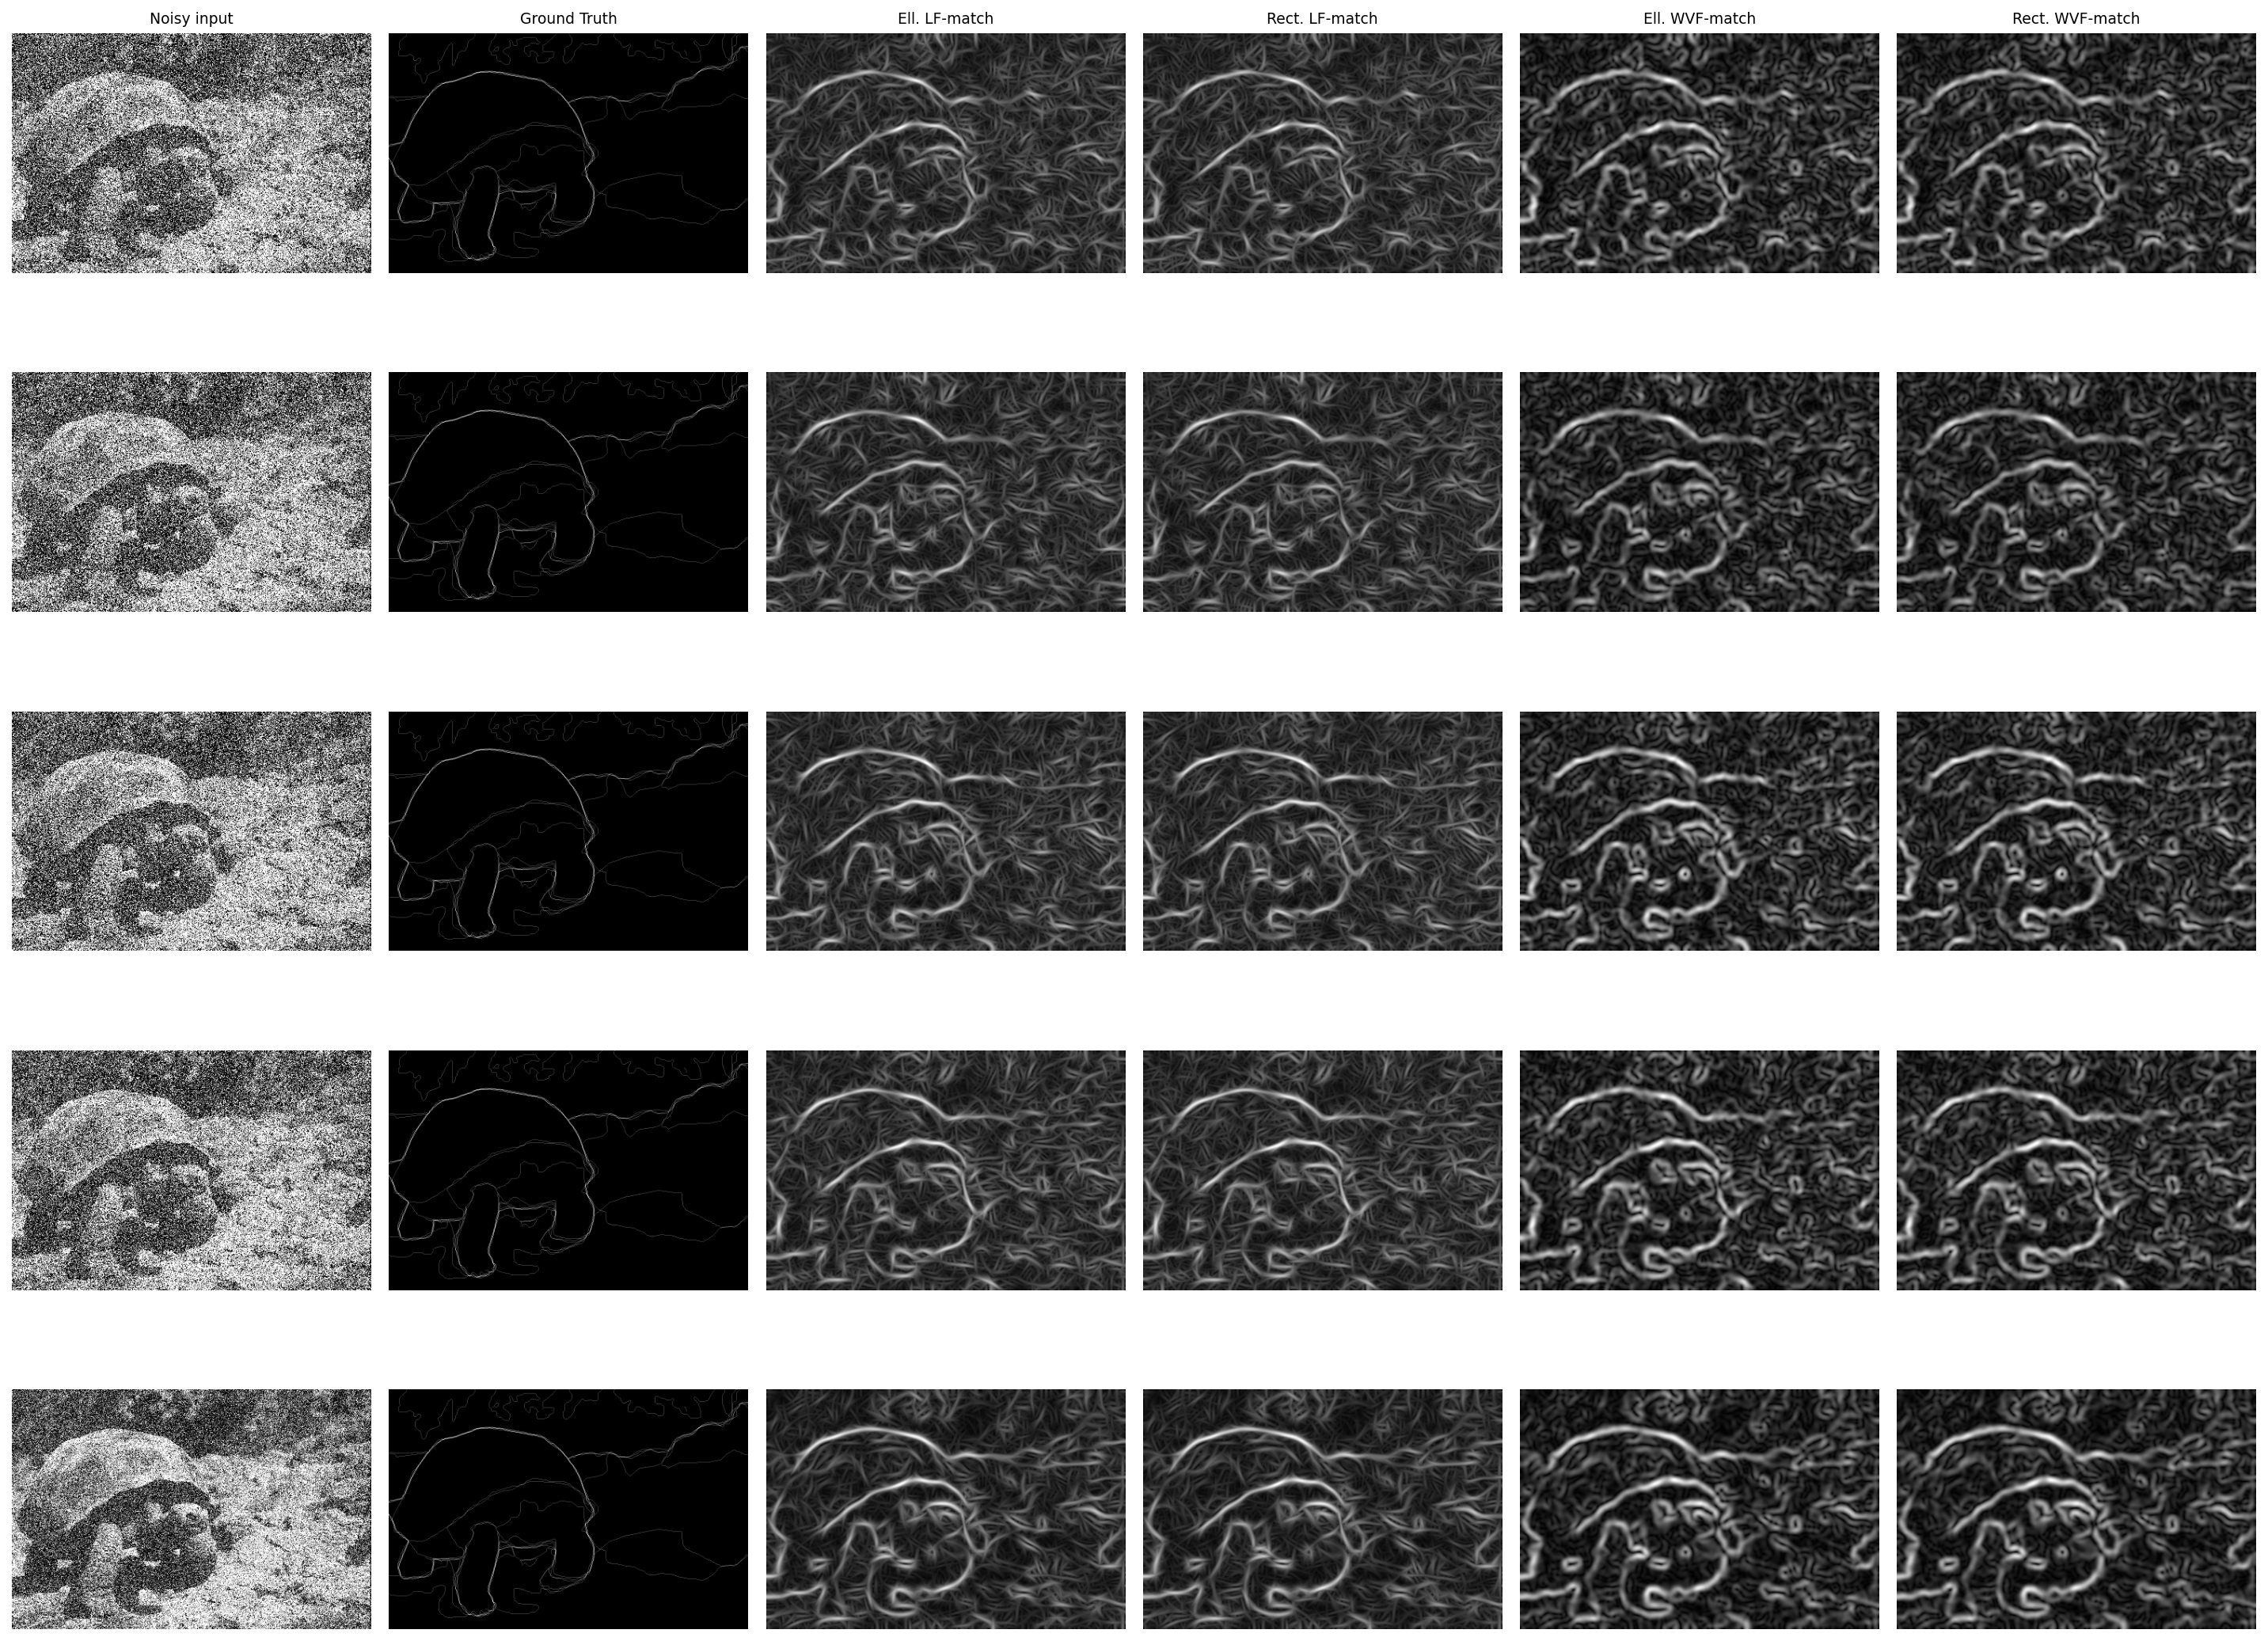
\includegraphics[width=0.92\textwidth]{BSDS500/noise_edgemaps_103006.png}
  \end{center}

  \vspace{0.1em}
  {\small Tortoise image. The elongated elliptical kernel (col 3) preserves edge structure even at SNR=0.3, where the circular WVF-matched kernels (cols 5--6) are visibly noisier.}
\end{frame}

% ============================================================
\sectionsubtitle{Matched to ablation-optimal ASF configurations}
\section{Ablation-Matched Results}

\begin{frame}{Matched to Optimal ASF Settings}
  The ASF ablation identified optimal configurations per dataset. We matched elliptical and rectangular kernels to each by measuring the fused stencil's pixel extent and deriving equivalent $\sigma$ values.

  \vspace{0.3em}
  \begin{center}
    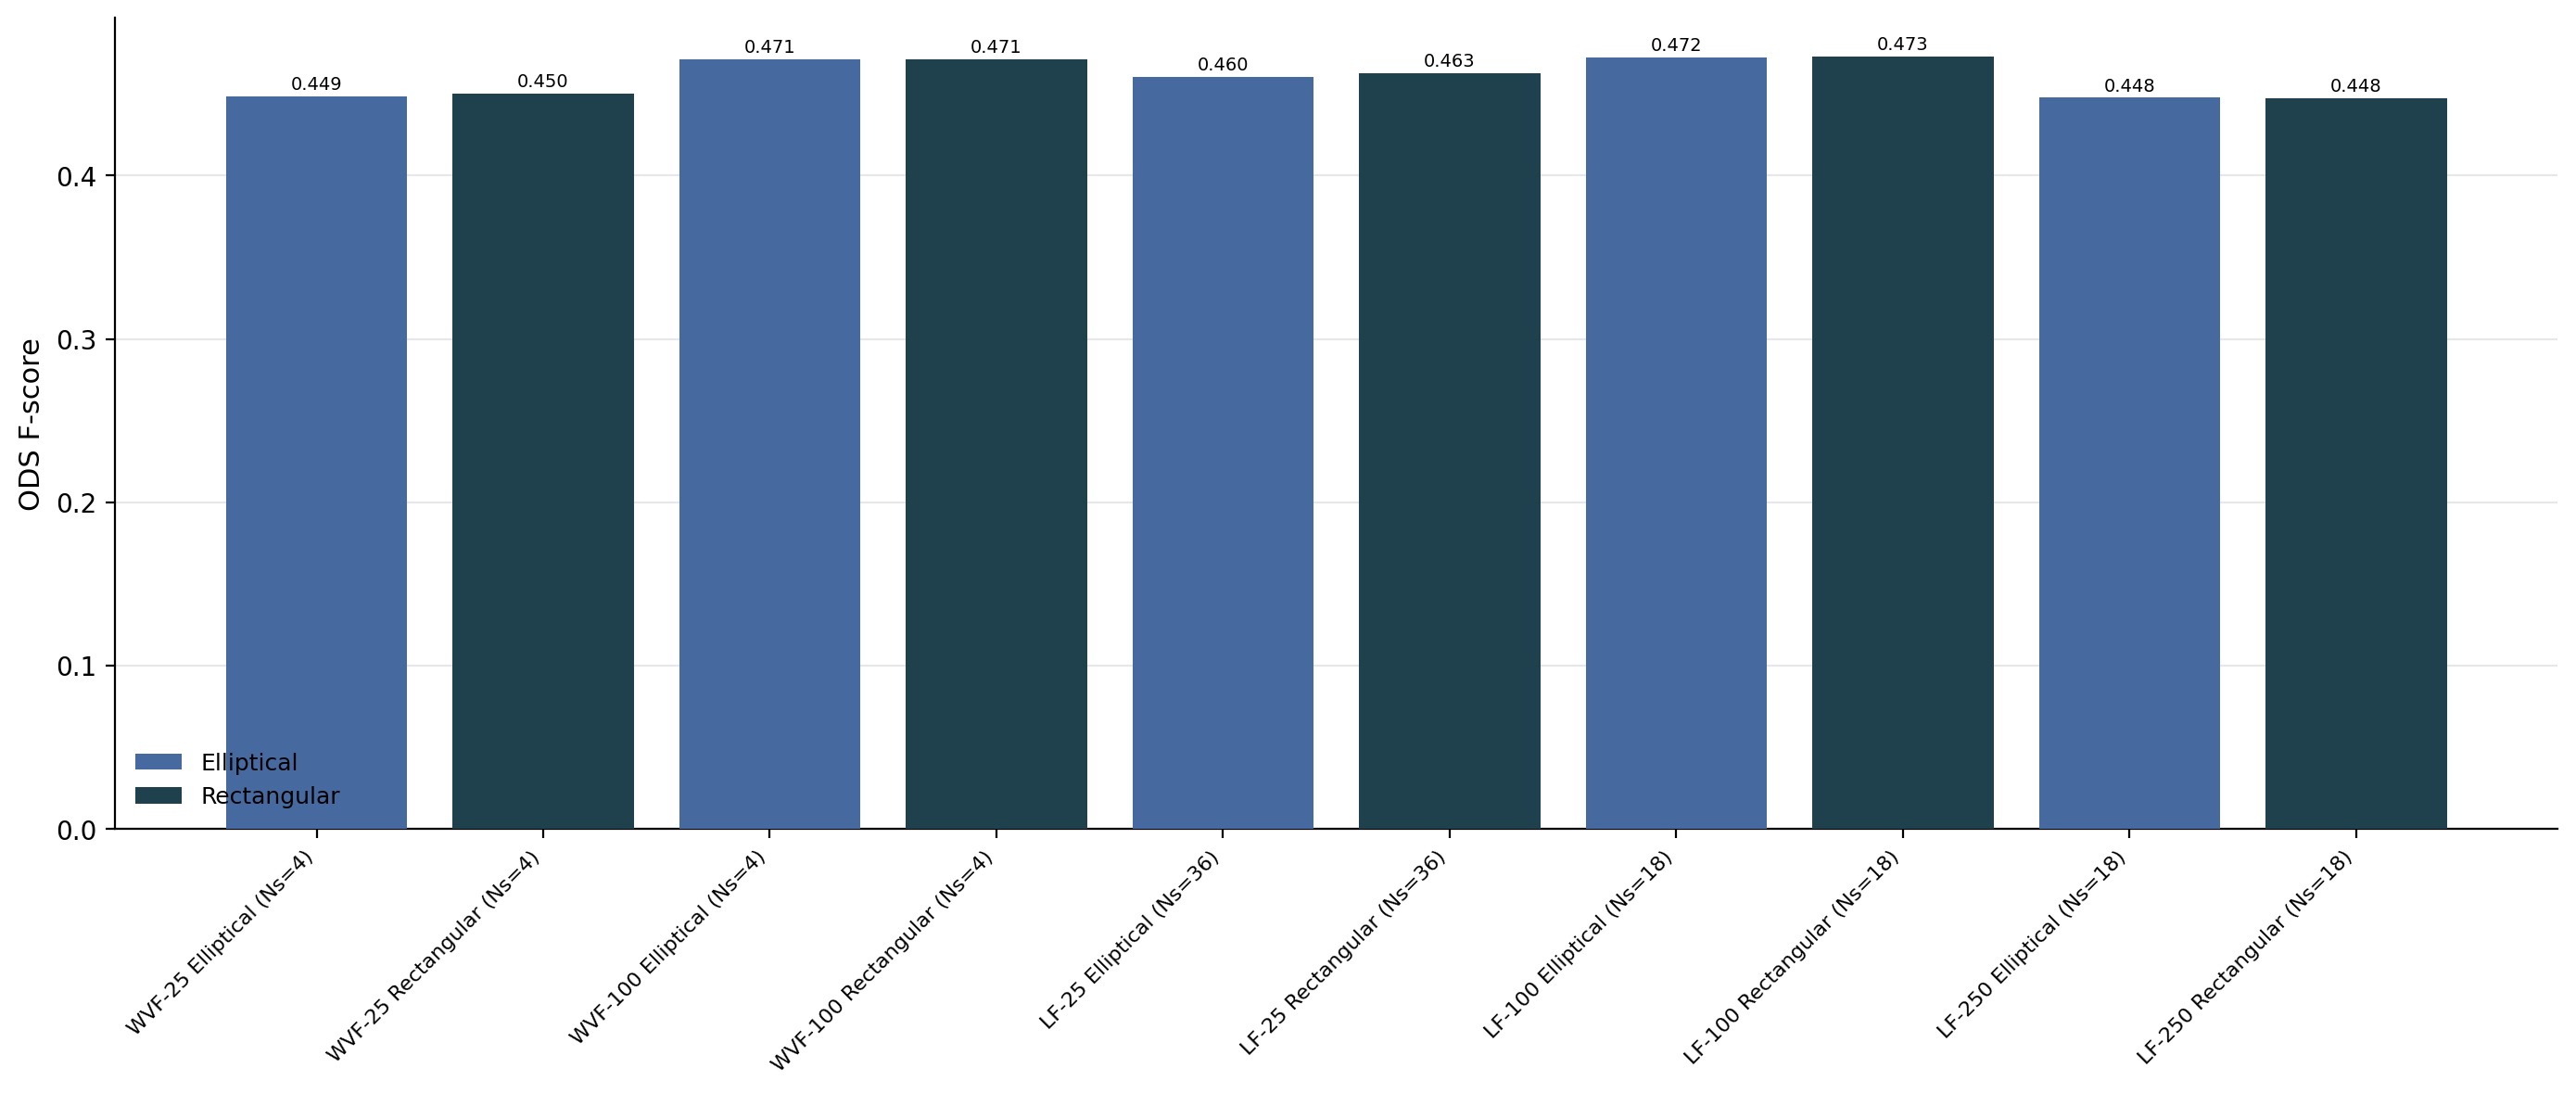
\includegraphics[width=0.82\textwidth]{BSDS500/matched_ablation_ods.png}
  \end{center}

  \vspace{0.1em}
  {\small Best performers: LF-100 match (Ns=18) and WVF-100 match (Ns=4) at $\sim$0.472 ODS. The WVF-100 match runs 2$\times$ faster with only 4 orientations.}
\end{frame}

% ============================================================
\sectionsubtitle{}
\section{Summary}

\begin{frame}{Summary}
  \textbf{The fused stencil's polynomial machinery is unnecessary for edge detection:}
  \begin{itemize}
    \item Overlapping virtual-pixel neighborhoods cancel weights and waste pixels
    \item 91--97 active pixels, many carrying near-zero weight
    \item Requires pseudoinverse, polynomial fitting, and deduplication
  \end{itemize}

  \vspace{0.5em}
  \textbf{Geometric kernels achieve the same accuracy with a simpler design:}
  \begin{itemize}
    \item Elliptical Gaussian: fewest pixels, cleanest weights, best under noise
    \item Rectangular Gaussian: slightly more pixels, marginally better on clean images
    \item Both are \textbf{3$\times$ faster} at matched parameters, with \textbf{$<$0.3\% ODS difference}
  \end{itemize}

  \vspace{0.5em}
  \textbf{Noise robustness is a function of kernel size, not polynomial order:}
  \begin{itemize}
    \item The original's small noise advantage vanishes when geometric kernels are scaled up
    \item Ablation confirms: heavy noise demands larger kernels and more orientations, not higher-order polynomial fits
  \end{itemize}
\end{frame}

% ------ Thank You / Q&A ------
{
  \setbeamertemplate{footline}{}
  \begin{frame}[plain]
    \begin{tikzpicture}[remember picture, overlay]
      \fill[UofSCGarnet] (current page.south west) rectangle (current page.north east);
      \fill[UofSCDarkGarnet] (current page.south west) rectangle ([yshift=0.8cm]current page.south east);
      \draw[white, line width=0.5pt] ([yshift=0.8cm]current page.south west) -- ([yshift=0.8cm]current page.south east);
    \end{tikzpicture}
    \vfill
    \centering
    {\fontsize{50}{55}\selectfont\impactfont\color{UofSCWhite} THANK YOU!}\\[1em]
    {\Large\color{UofSCWhite} Questions \& Discussion}\\[0.5em]
    {\normalsize\color{UofSCGray30} vaught@email.sc.edu}
    \vfill
  \end{frame}
}

\end{document}
